%% Template article for Elsevier's document class `elsarticle'
%% with numbered style bibliographic references
%% SP 2008/03/01

% \documentclass[preprint,12pt]{elsarticle}

%% Use the option review to obtain double line spacing
% \documentclass[authoryear,preprint,review,12pt]{elsarticle}

%% Use the options 1p,twocolumn; 3p; 3p,twocolumn; 5p; or 5p,twocolumn
%% for a journal layout:
% \documentclass[final,1p,times]{elsarticle}
% \documentclass[final,1p,times,twocolumn]{elsarticle}
% \documentclass[final,3p,times]{elsarticle}

% \documentclass[final,3p,times,twocolumn,authoryear]{elsarticle}
\documentclass[preprint,review,3p,times,onecolumn,authoryear]{elsarticle}

%% \documentclass[final,5p,times]{elsarticle}
%% \documentclass[final,5p,times,twocolumn]{elsarticle}

%% For including figures, graphicx.sty has been loaded in
%% elsarticle.cls. If you prefer to use the old commands
%% please give \usepackage{epsfig}

%% The amssymb package provides various useful mathematical symbols
\usepackage{amssymb}
%% The amsthm package provides extended theorem environments
%% \usepackage{amsthm}

%% The lineno packages adds line numbers. Start line numbering with
%% \begin{linenumbers}, end it with \end{linenumbers}. Or switch it on
%% for the whole article with \linenumbers.
\usepackage{lineno}

\journal{Computers \& Geosciences}


%%%%%%%%%%%%%%%%%%%%%%%%%%%%%%%%%%%%%%%%%%%%%
\usepackage{xspace,color,amsmath}
% \usepackage{minted}

\usepackage{enumitem}
\setitemize{noitemsep,topsep=0pt,parsep=0pt,partopsep=0pt}

\newcommand{\SimPEG}{\textsc{SimPEG}\xspace}
\newcommand{\simpegEM}{\textsc{simpegEM}\xspace}

\newcommand{\Mesh}{\texttt{Mesh}\xspace}
\newcommand{\Survey}{\texttt{Survey}\xspace}
\newcommand{\DCSurvey}{\texttt{DCSurvey}\xspace}
\newcommand{\Problem}{\texttt{Problem}\xspace}
\newcommand{\DCProblem}{\texttt{DCProblem}\xspace}
\newcommand{\EMProblem}{\texttt{EMProblem}\xspace}
\newcommand{\Regularization}{\texttt{Regularization}\xspace}
\newcommand{\DataMisfit}{\texttt{DataMisfit}\xspace}
\newcommand{\Optimization}{\texttt{Optimization}\xspace}
\newcommand{\InvProblem}{\texttt{InvProblem}\xspace}
\newcommand{\Inversion}{\texttt{Inversion}\xspace}

\newcommand{\dobs}{\mathbf{d}_\text{obs}}
\newcommand{\m}{\mathbf{m}}
\newcommand{\du}{\mathbf{u}}
\newcommand{\mref}{\mathbf{m}_\text{ref}}
\newcommand{\dpred}{\mathbf{d}_\text{pred}}
\newcommand{\meshI}{\emph{mesh}$_I$\xspace}
\newcommand{\meshF}{\emph{mesh}$_F$\xspace}
\newcommand{\Wd}{\mathbf{W}_\text{d}}
\newcommand{\Wm}{\mathbf{W}_\text{m}}

\newcommand{\deriv}[2]{\frac{d #1}{d #2}}

\newcommand{\minimize}[1]{\mathop{\hbox{minimize}}_{#1}}

\renewcommand{\div}{\nabla\cdot\,}
\newcommand{\grad}{\vec \nabla}
\newcommand{\curl}{{\vec \nabla}\times\,}
\newcommand {\J}{{\vec J}}
\renewcommand{\H}{{\vec H}}
\newcommand {\E}{{\vec E}}
\newcommand{\dcurl}{{\mathbf C}}
\newcommand{\dgrad}{{\mathbf G}}
\newcommand{\Acf}{{\mathbf A_c^f}}
\newcommand{\Ace}{{\mathbf A_c^e}}
\renewcommand{\S}{{\mathbf \m}}
\newcommand{\St}{{\mathbf \Sigma_\tau}}
\newcommand{\T}{{\mathbf T}}
\newcommand{\Tt}{{\mathbf T_\tau}}
\newcommand{\diag}[1]{\,{\sf diag}\left( #1 \right)}
\newcommand{\M}{{\mathbf M}}
\newcommand{\MfMui}{{\M^f_{\mu^{-1}}}}
\newcommand{\MeSig}{{\M^e_\sigma}}
\newcommand{\MeSigInf}{{\M^e_{\sigma_\infty}}}
\newcommand{\MeSigO}{{\M^e_{\sigma_0}}}
\newcommand{\Me}{{\M^e}}
\newcommand{\Mes}[1]{{\M^e_{#1}}}
\newcommand{\Mee}{{\M^e_e}}
\newcommand{\Mej}{{\M^e_j}}
\newcommand{\BigO}[1]{\mathcal{O}\bigl(#1\bigr)}
\newcommand{\bE}{\mathbf{E}}
\newcommand{\bH}{\mathbf{H}}
\newcommand{\B}{\vec{B}}
\newcommand{\D}{\vec{D}}
\renewcommand{\H}{\vec{H}}
\newcommand{\s}{\vec{s}}
\newcommand{\bfJ}{\bf{J}}
\newcommand{\vecm}{\vec m}
\renewcommand{\Re}{\mathsf{Re}}
\renewcommand{\Im}{\mathsf{Im}}
\renewcommand {\j}  { {\vec j} }
\newcommand {\h}  { {\vec h} }
\renewcommand {\b}  { {\vec b} }
\newcommand {\e}  { {\vec e} }
\newcommand {\db}  { {\mathbf {b}} }
\newcommand {\de}  { {\mathbf {e}} }
\renewcommand {\d}  { {\vec d} }
\renewcommand {\u}  { {\mathbf u} }
\newcommand{\I}{\vec{I}}
%%%%%%%%%%%%%%%%%%%%%%%%%%%%%%%%%%%%%%%%%%%%%
\usepackage{etoolbox}
\newtoggle{finaldraft}
\togglefalse{finaldraft}


\begin{document}

\begin{frontmatter}

%% Title, authors and addresses

%% use the tnoteref command within \title for footnotes;
%% use the tnotetext command for theassociated footnote;
%% use the fnref command within \author or \address for footnotes;
%% use the fntext command for theassociated footnote;
%% use the corref command within \author for corresponding author footnotes;
%% use the cortext command for theassociated footnote;
%% use the ead command for the email address,
%% and the form \ead[url] for the home page:
%% \title{Title\tnoteref{label1}}
%% \tnotetext[label1]{}
%% \author{Name\corref{cor1}\fnref{label2}}
%% \ead{email address}
%% \ead[url]{home page}
%% \fntext[label2]{}
%% \cortext[cor1]{}
%% \address{Address\fnref{label3}}
%% \fntext[label3]{}

{%\iftoggle{finaldraft}{
\title{\SimPEG: An open source framework for simulation and gradient based
parameter estimation in geophysical applications}

%% use optional labels to link authors explicitly to addresses:
\author[UBC1]{Rowan Cockett}
\author[UBC]{Seogi Kang}
\author[UBC]{Lindsey J. Heagy}
\author[UofC]{Adam Pidlisecky}
\author[UBC]{Douglas W. Oldenburg}

\address[UBC1]{Corresponding Author. Phone: 1(604)358-7696, Email: rcockett[at]eos.ubc.ca}
\address[UBC]{Geophysical Inversion Facility, University of British Columbia}
\address[UofC]{University of Calgary}

\begin{abstract}

Inverse modeling is a powerful tool for extracting information about the subsurface from geophysical data. Geophysical inverse problems are inherently multidisciplinary, requiring elements from the relevant physics, numerical simulation, and optimization, as well as knowledge of the geologic setting, and a comprehension of the interplay between all of these elements. The development and advancement of inversion methodologies can be enabled by a framework that supports experimentation, is flexible and extensible, and allows the knowledge generated to be captured and shared. The goal of this paper is to propose a framework that supports many different types of geophysical forward simulations and deterministic inverse problems. Additionally, we provide an open source implementation of this framework in Python called \SimPEG (Simulation and Parameter Estimation in Geophysics, http://simpeg.xyz). Included in \SimPEG are staggered grid, mimetic finite volume discretizations on a number of structured and semi-structured meshes, convex optimization programs, inversion routines, model parameterizations, useful utility codes, and interfaces to standard numerical solver packages. The framework and implementation are modular, allowing the user to explore, experiment with, and iterate over a variety of approaches to the inverse problem. \SimPEG provides an extensible, documented, and well-tested framework for inverting many types of geophysical data and thereby helping to answer questions in geoscience applications. Throughout the paper we use a generic direct current resistivity problem to illustrate the framework and functionality of \SimPEG.
\end{abstract}

\begin{keyword}
Geophysics; Numerical modeling; Inversion; Electromagnetics; Sensitivities; Object-oriented programming;
\end{keyword}
}

\end{frontmatter}

\linenumbers

\section{Introduction and Motivation}
\label{sec:intro}

Geophysical surveys can be used to obtain information about the subsurface as the responses that are measured depend on the physical properties and contrasts in the earth. Inversions provide a mathematical framework for constructing physical property models consistent with the data collected by these surveys. The data collected are finite in number while the physical property distribution of the earth is continuous. Thus, inverting for a physical property model from geophysical data is an ill-posed problem, meaning that no unique solution explains the data. Furthermore, the data may be contaminated with noise. Therefore, the goal of a deterministic inversion is not only to find a model consistent with the data, but must be to find the `best' model that is consistent with the data\footnote{Alternatively, the inverse problem can be formulated in a probabilistic framework, see for example \citep{Tarantola2015,Tarantola1982}. In this paper we will focus our attention on the deterministic approach.}. The definition of `best' requires the incorporation of assumptions and \emph{a priori} information, often in the form of an understanding of the particular geologic setting or structures \citep{Constable1987, DougTutorial, lelievre2009integrating}. Solving the inverse problem involves many moving pieces that must work together, including physical simulations, optimization, linear algebra, and incorporation of geology. Deterministic geophysical inversions have been extensively studied, and many components and methodologies have become standard practice. With increases in computational power and instrumentation quality, there is a greater drive to extract more information from the geophysical data. Additionally, geophysical surveys are being applied in progressively more challenging environments. As a result, the geosciences are moving towards the integration of geological, geophysical, and hydrological information to better characterize the subsurface (e.g. \cite{ho,Doetsch2010,Gao2012}). This is a scientifically and practically challenging task \citep{Li2000a, lelievre2009integrating}. These challenges, compounded with inconsistencies between different data sets, often makes the integration and implementation complicated and/or non-reproducible. The development of new methodologies to address these challenges will build upon, as well as augment, standard practices; this presupposes that researchers have access to consistent, well-tested tools that can be extended, adapted and combined.

There are many proprietary codes available that focus on efficient algorithms and are optimized for a specific geophysical application (e.g. \cite{Kelbert2014a, Key2007, liol96, Li1998a}). These packages are effective for their intended application, for example, a domain specific large-scale geophysical inversion or a tailored industry workflow. However, many of these packages are `black-box' algorithms, that is, they cannot easily be interrogated or extended. As researchers, we require the ability to interrogate and extend ideas; this must be afforded by the tools that we use.
Accessibility and extensibility are the primary motivators for this work.
Other disciplines have approached the development of these tools through open source initiatives using interpreted languages, such as Python, for example, Astropy in astronomy \citep{Astropy} and SciPy in numerical computing \citep{scipy}. Interpreted languages facilitate interactive development using scripting, visualization, testing, and interoperability with code in compiled languages and existing libraries. Furthermore, many open source initiatives have led to communities with hundreds of researchers contributing and collaborating using social coding platforms, such as GitHub (https://github.com). There are also initiatives in the geophysical forward and inverse modeling community targeting specific geophysical applications (cf. \cite{Hansen2013, PySIT2013, Uieda2014, Kelbert2014a, Modflow}). We are interested in creating a community around geophysical simulations and gradient based inversions. To create a foundation on which to build a community, we require a comprehensive framework that is applicable across domains and upon which researchers can readily develop their own tools and methodologies. To support these goals, this framework must be modular and its implementation must be easily extensible by researchers.

The goal of this paper is to present a comprehensive framework for simulation and gradient based parameter estimation in geophysics. The core ideas from a variety of geophysical inverse problems have been distilled to create this framework. We also provide an open source library written in Python called \SimPEG (Simulation and Parameter Estimation in Geophysics, http://github.com/simpeg/simpeg). Our implementation has core dependencies on SciPy, NumPy, and Matplotlib, which are standard scientific computing packages in Python \citep{scipy, python, scipyOliphant, Hunter:2007}. \SimPEG includes staggered grid, mimetic finite volume discretizations on structured and semi-structured meshes. It interfaces to standard numerical solver packages, convex optimization algorithms, model parameterizations, and visualization routines. We make use of Python's object-oriented paradigm leading to modular code that is extensible through inheritance and subtype polymorphism. \SimPEG follows a fully open source development paradigm \citep{Feller2000}, and uses the permissive MIT license. Throughout its development, we have focused on modularity, usability, documentation, and extensive unit-testing \citep{Wilson2014, RTFD, Travis, Coveralls}. Please see the website (http://simpeg.xyz) for up-to-date code, examples and documentation of this package; in addition see \cite{Kang2014, KangSEG2015, Kang2015, Kang2015a, HeagySEG2014, HeagySEG2015} for examples of research and use cases throughout a variety of geophysical applications. We hope that the organization, modularity, minimal dependencies, documentation, and testing in \SimPEG will encourage reproducible research, cooperation, and communication to help tackle some of the inherently multidisciplinary geophysical problems.

\bigskip

To guide the discussion, we start this paper by outlining gradient based inversion methodology in Section~\ref{sec:methodology}. The inversion methodology directly motivates the construction of the \SimPEG framework, terminology, and software implementation which we discuss in Section~\ref{sec:implementation}. We weave an example of Direct Current (DC) resistivity throughout the discussion of the \SimPEG framework to provide context for the choices made and highlight many of the features of \SimPEG.


\section{Inversion Methodology}
\label{sec:methodology}

Geophysical inverse problems are motivated by the desire to extract information about the earth from measured data.
A typical geophysical datum can be written as
{%\iftoggle{finaldraft}{
\begin{equation}
\label{eq:genericdatum}
F_i[\m] + \epsilon_i= d_i,
\end{equation}
}
where $F$ is a forward simulation operator that incorporates details of the
relevant physical equations, sources, and survey design, $\m$ is a generic
symbol for the inversion model, $\epsilon_{i}$ is the noise that is often assumed to have known statistics,
and $d_i$ is the observed datum.
In a typical geophysical survey we are provided with the data $d_i, i=1...N$ and
some estimate of their uncertainties. The goal
is to recover the model, $\m$, which is often a physical property. The data provide only a
finite number of inaccurate constraints upon the sought model.
Finding a model from the data alone is an ill-posed problem since there is no unique model that explains the data.
Additional information must be included using prior information and assumptions,
for example, downhole property logs, structural orientation information, or known interfaces \citep{Fullagar2008,Li2000,lelievre2009integrating}.
This prior knowledge is crucial if we are to obtain an appropriate
representation of the earth, and will be discussed in more detail in Section~\ref{sub:inputs}.


Defining a well-posed inverse problem and solving it is a complex task that
requires many components that must interact. It is helpful to view this task as a workflow in which various
elements are explicitly identified and integrated. Figure~\ref{fig:inversionOutline}
outlines the inversion methodology that consists of inputs, implementation, and evaluation. The
inputs are composed of the geophysical data, the equations which are a mathematical
description of the governing physics, and prior knowledge or assumptions about the
setting. The implementation consists of two broad categories: the forward simulation
and the inversion. The forward simulation is the means by which we solve the
governing equations given a model and the inversion components evaluate and update this model.
We are considering a gradient based approach, which updates the model through an optimization routine.
The output of this implementation is a model, which, prior to interpretation, must be evaluated. This requires considering, and often re-assessing, the choices and assumptions made in both the input and implementation stages.
In this paper we are primarily concerned with the implementation component, that is,
how the forward simulation and inversion are carried out numerically. As a prelude
to discussing how the \SimPEG software is implemented, we step through the elements
in Figure~\ref{fig:inversionOutline} considering a Tikhonov-style inversion.

{%\iftoggle{finaldraft}{
\begin{figure}[ht!]
\centering
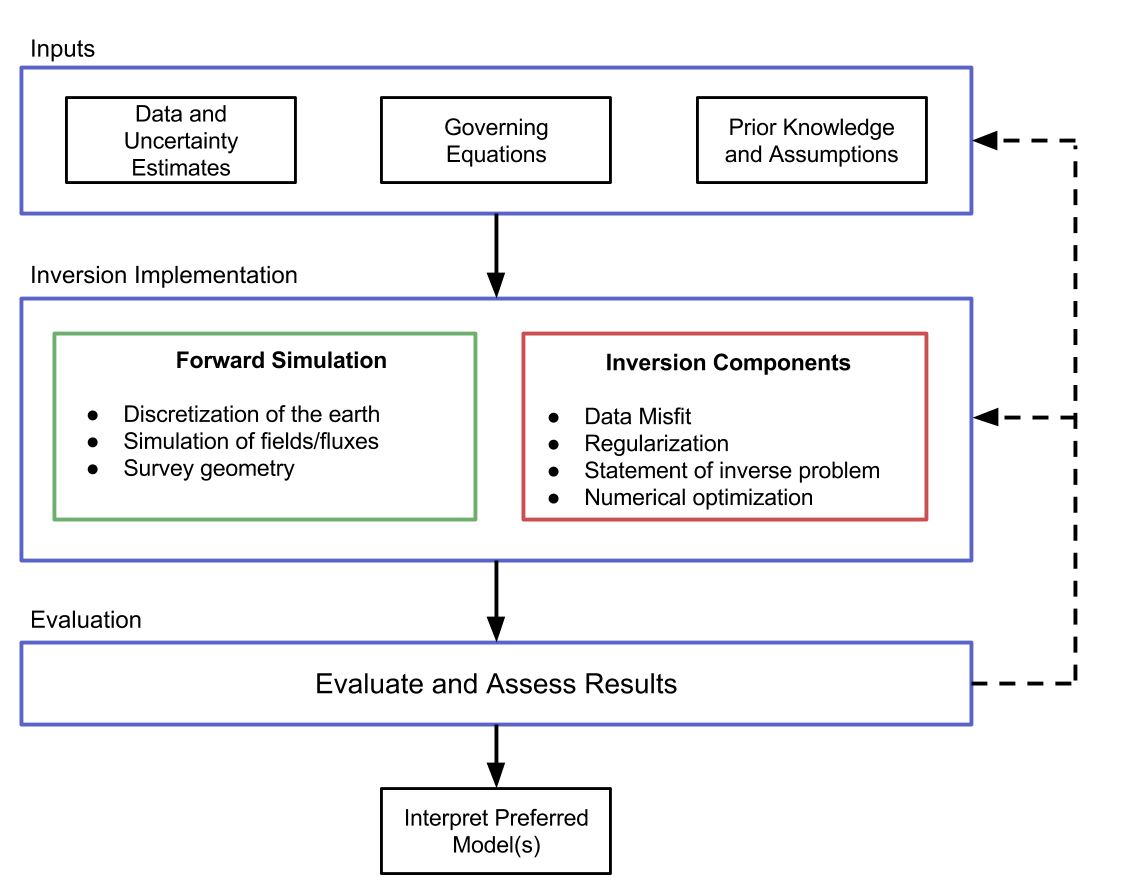
\includegraphics[width=7.5cm]{images/InversionWorkflowBulletsv2.png}
\caption{Inversion methodology. Including inputs, implementation, evaluation and interpretation. }
\label{fig:inversionOutline}
\end{figure}
}

\subsection{Inputs}
\label{sub:inputs}

Three sources of input are required prior to performing an inversion:
(1) the geophysical data and uncertainty estimates,
(2) the governing equations that connect the sought model with the observations, and
(3) prior knowledge about the model and the context of the problem.
%that inversion will help solve.

\subsubsection*{Data and uncertainty estimates}

At the heart of the inversion are the geophysical data that consist of
measurements over the earth. These data depend on the type of survey,
the physical property distribution, and the type and location of
the measurements. The details about the survey, for example the location, orientation and waveform of a source, and which component
of a particular wavefield is measured at a receiver, must be known.
The data are contaminated with additive noise which can sometimes be
estimated by taking multiple realizations of the data.
However, standard deviations of those realizations only provide a lower bound for the noise.
% those provide only a lower bound.
For the
inverse problem, the uncertainty in the data must include not only this
additive noise, but also any discrepancy between the true earth experiment
and our mathematical representation of the data. This requires
accounting for mislocation of receivers and sources,
poor control of the transmitter waveform, electronic gains
or filtering applied to signals entering the receivers, incorrect
dimensionality in our mathematical model (e.g. working in 2D instead of 3D),
neglect of physics in our mathematical equations by introducing assumptions (e.g. using a straight ray tomography vs. a full waveform simulation in seismic), and discretization errors of
our mathematical equations.

\subsubsection*{Governing equations}

The governing equations provide the connection between the physical properties
of the subsurface and the data we observe.
Most frequently, these are sets of partial differential equations with specific
boundary conditions.
The governing equations, with specified source terms,
can be solved through numerical discretization using
finite volume, finite element, or integral equation techniques.
Alternatively, they may also be solved
through evaluations of analytic functions.
Whichever approach is taken, it is crucial that there exists some way to
simulate the data response given a model.

\subsubsection*{Prior knowledge}

If there is one model that acceptably fits the data then there are
infinitely many. Additional information is therefore required to reduce the non-uniqueness.
This can be geologic information, petrophysical knowledge about the various rock types, borehole logs,
additional geophysical data sets, or inversion results. This prior information
can be used to construct reference models for the inversion and also
characterize features of the model, such as whether it is best described by a smooth function
or if it is discontinuous across interfaces. Physical property measurements
can be used to assign upper and lower bounds for a physical property model at
points in a volume or in various regions within our 3D volume.
The various types of information that are relevant to the geologic and
geophysical questions to be addressed must be combined
and translated into useful information for the inversion \citep{lelievre2009integrating,MaokunLi2010}.

\subsection{Implementation}

In this section we outline the components necessary to formulate a well-posed inverse problem and solve it
numerically.
Two major abilities are critical to running the inversion:
(1) the ability to simulate data, and
(2) the ability to assess and update the model (Figure~\ref{fig:inversionOutline}).
% In , we highlight the components
% involved in the implementation of the inversion, namely forward simulation and parameter estimation (inversion).
% Something about both of these abilities being in the same framework.

%%%%%%%%%%%%%%%%%%%%%%%%%%%%%%%%%%%%
%%%%%%    Forward Simulation  %%%%%%
%%%%%%%%%%%%%%%%%%%%%%%%%%%%%%%%%%%%
\subsubsection*{Forward simulation}
The ability to carry out an inversion presupposes the ability to run a
forward simulation and create predicted data given a physical property model.
In forward simulation, we wish to compute $F[\m]=\dpred$. The operator $F$
simulates the specific measurements taken in a geophysical survey using the governing equations.
The survey refers to all details regarding the field experiment that are needed
to simulate the data. The forward simulation
of DC resistivity data requires knowledge of the topography, the resistivity of the earth,
and the survey details including locations of the current and potential electrodes, the source waveform, and
the units of the observations. % (e.g. Volts or millivolts),
%polarity of data, %(since negative and positive electrodes can sometimes be interchanged in the field)
%and the topography of the survey area.
To complete the simulation, we need to solve our governing equations
using the physical property model, $\m$, that is provided.
In the DC resistivity experiment, our partial differential equation with supplied boundary conditions
is solved with an appropriate numerical method, for example, finite volumes, finite elements, integral equations,
or semi-analytic methods for 1D problems.
In any case, we must discretize the earth onto a numerical forward simulation mesh (\meshF) that is appropriate.
The size of the cells will depend upon the structure of the physical property model, topography,
as well as the distance between sources and receivers.
Cells in \meshF must be small enough, and the domain large enough,
so that sufficient numerical accuracy is achieved.
Proper mesh design is crucial so that numerical modeling errors are below a prescribed threshold value (cf. \cite{haber2015computational}).


In general, we can write our governing equations in the form of
{%\iftoggle{finaldraft}{
\begin{equation}
\label{eq:fwdmodel}
C(\m,\u) = 0,
\end{equation}
}
where $\m$ is the modeled physical property, $\u$ are the fields and/or fluxes.
$C$ is often given by a partial differential equation or a set of partial
differential equations. Information about the sources and appropriate boundary
conditions are included in $C$. This system is solved for $\u$
and the predicted data are extracted from $\u$ via a projection (or functional), $\dpred = P[\u]$.
The ability to simulate the geophysical problem and generate predicted data
is a crucial building block. Accuracy and efficiency are essential since many
forward problems must be evaluated when carrying out any inversion.

%%%%%%%%%%%%%%%%%%%%%%%%%%%%%%%%%%%%
%%%%%%%  Essential Elements  %%%%%%%
%%%%%%%%%%%%%%%%%%%%%%%%%%%%%%%%%%%%
\subsubsection*{Inversion elements}

%%%%%%%%%%%%%%%%%%%%%%%%%%%%%%%%%%%%
%%%%%%    Parameterization    %%%%%%
%%%%%%%%%%%%%%%%%%%%%%%%%%%%%%%%%%%%

In the inverse problem, the first step is to specify how we parameterize the
earth model. Finding a distributed physical property can be done by
discretizing the 3D earth into voxels, each of which has a constant but unknown value.
It is convenient to refer to the domain on which this model is discretized as the inversion mesh, \meshI.
The choice of discretization involves an assessment of the expected dimensionality of
the earth model. If the physical property varies only with depth, then
the cells in \meshI can be layers and a 1D inverse problem can be formulated. A more
complex earth may require 2D or 3D discretizations.
The choice of discretization depends on the spatial distribution and resolution of the
data and the expected complexity of the geologic setting.
We note that the inversion mesh has different design criteria and constraints than the
forward simulation mesh. For convenience, many inverse problems have
historically been solved with \meshI = \meshF so that only one discretization is needed for the inversion.
There is a growing body of work that investigates combinations of inversion discretizations and
forward modeling meshes that are geared towards
problem specific formulations % talking about object based inversions/parameterizations
as well as efficiency in large-scale problems \citep{Haber2014,Yang2014, HaHe06}. % multi meshes, dikun, eldadOctree
In any formulation there exists a mapping between \meshI and \meshF such that the
parameterization chosen can be used to simulate data in a forward simulation.

To formulate a mathematical statement of the inverse problem, there are two essential elements:
\begin{enumerate}
    \item \emph{data misfit}: a metric that measures the misfit between the observed and predicted data; and
    \item \emph{regularization}: a metric that is constructed to evaluate the model's agreement with assumptions and prior knowledge.
\end{enumerate}

\bigskip

The data misfit requires an assessment of the
error in each datum. These errors result from anything that yields a discrepancy between the
mathematical modeling and the true value. It includes additive noise, errors in the description of survey parameters (eg. receiver locations, transmitter waveforms, etc.),
incorrect choice of governing equations, and numerical
errors arising from the simulation technique. Clearly, quantifying the noise
for each datum is a challenge.

The data misfit is a measure of how well the data predicted by a given
model reproduce the observed data. To assess \emph{goodness of fit}, we select a norm which evaluates the `size' of the misfit. This metric must include an uncertainty estimate for each datum. Often we assume that the data errors are Gaussian and uncorrelated and then estimate the standard deviation for each datum. The most common norm, and one that is compatible with Gaussian statistics, has the form:
{%\iftoggle{finaldraft}{
\begin{equation}
\label{eq:phid}
  \phi_d(\m) = \frac{1}{2}\|\Wd (F[\m] - \dobs) \|^2_2.
\end{equation}
}
Here $F[\m]$ is a forward modeling that produces predicted data $\dpred$, as in equation \ref{eq:genericdatum}.
$\Wd$ is a diagonal matrix whose elements are equal to ${\bf W}_{d_{ii}}=1/\epsilon_i$ where
$\epsilon_i$ is an estimated standard deviation of the $i$\textsuperscript{th} datum. It is
important to give careful thought into assignment of these. A good
option is to assign a $\epsilon_i = floor + \%|d_i|$.
Percentages are generally required when there is a large dynamic
range of the data. A percentage alone can cause great difficulty
for the inversion if a particular datum acquires a value close to zero, and therefore we include a floor.

In addition to a metric that evaluates the size of the misfit, it is also
required that we have a tolerance, $\phi_d^*$; models satisfying $\phi_d(\mathbf{m}) \leq \phi_d^*$ are considered to adequately fit the data \citep{parker1994geophysical}. If the data errors are Gaussian and
we have assigned the correct standard deviations, then the expected value of
$\phi_d^* \approx N$, where $N$ is the number of data. Finding a model that has a misfit
substantially lower than this will result in a solution that has excessive
and erroneous structure, that is, we are fitting the noise. Finding a model that has
a misfit substantially larger than this will yield a model that is
missing structure that could have been extracted from the data (see \cite{DougTutorial} for a tutorial).

The choice of misfit in equation \ref{eq:phid} is not the only possibility for a misfit measure.
If data errors are correlated, then $\Wd$ is the square root of the data covariance
matrix and it will have off-diagonal terms. Often useful in practice is recognizing
if the noise statistics are non-Gaussian. Incorporating robust statical measures,
like $l_p$ norms with $p\approx1$, are useful for handling outliers \citep{ekblom1973calculation,Farquharson1998}.

\bigskip

The second essential inversion element is defining the regularization functional.
If there is one model that has a misfit that equals the desired tolerance,
then there are infinitely many other models which can fit to the same
degree. The challenge is to find that model which has the desired characteristics
and is compatible with \emph{a priori} information. A single model can be selected
from an infinite ensemble by measuring the length, or norm, of each model.
Then a smallest, or sometimes largest, member can be isolated. Our goal is to design a norm
that embodies our prior knowledge and, when minimized,
yields a realistic candidate for the solution of our problem. The norm can
penalize variation from a reference model, spatial derivatives of the model, or
some combination of these.
We denote this norm by $\phi_m$ and write it in a matrix form, for example,
{%\iftoggle{finaldraft}{
\begin{equation}
\label{eq:phim}
\phi_m(\m)= \frac{1}{2}\|\Wm(\m-\mref)\|^2_2.
\end{equation}
}
$\mathbf{W_m}$ is a matrix and $\mref$ is a reference model (which could be zero).
The matrix $\mathbf{W_m}$ can be a stacked combination of matrices weighted by $\alpha_*$:
{%\iftoggle{finaldraft}{
\begin{equation}
\label{eq:Wm}
    \bf \Wm = [\alpha_s I, \quad \alpha_x W_x^\top, \quad \alpha_y W_y^\top, \quad \alpha_z W_z^\top]^\top.
\end{equation}
}
Here $\Wm$ is a combination of smallness and first-order smoothness in the $x$, $y$, and $z$ directions.
Each of the $\bf W$ matrices is, in fact, a discrete representation of an integral (cf. \cite{DougTutorial}) .
The final regularization $\Wm$ can be a weighted sum of these, with $\alpha_*$ being applied as scalars or diagonal matrices with varying weights for each cell or cell face (cf. \cite{DougTutorial,haber2015computational}).
%When working in 3D volumes, each regularization functional is a discrete representation of an integral (CITE).
Additional weightings can also be incorporated through $\Wm$, such as depth weighting, which is important in
potential field inversions (such as magnetics and gravity), or sensitivity weightings to prevent model structure from
concentrating close to sources or receivers \citep{li19963,li2000joint}.
% Some examples are:
% \begin{equation}
% \begin{split}
% \int \left( \mathbf{w_s} (\mathbf{m-m}_{ref})\right)^2 dV ~~ \quad \text{    (smallness)},& \\
% \int \left( \mathbf{w_x} \deriv{\bf m}{x}\right)^2 dV \quad \quad \quad \text{(x-smoothness)},& \\
% \int \left( \mathbf{w_y} \deriv{\bf m}{y}\right)^2 dV \quad \quad \quad \text{(y-smoothness)},&\\
% \int \left( \mathbf{w_z} \deriv{\bf m}{z}\right)^2 dV \quad \quad \quad \text{(z-smoothness)},&
% \end{split}
% \end{equation}
The regularization functionals addressed provide constraints on the model
in a weak form, that is, a single number is used to characterize the entire model.
Strong constraints that work within each cell can often be provided
in the form of upper and lower bounds; these will be incorporated in the following section.
The $l_2$ norms referred to above are appropriate for many problems, however models norms,
such as $l_p$-norms, total variation, minimum support stabilizing functionals, or rotated smoothness operators that favor different character and~/~or include
additional information can also be designed (cf. \cite{oldenburg1984introduction,DougTutorial,claerbout1973robust,strong2003edge,Zhdanov2002,Li2000}).
% For example
% \begin{equation}
% \int |\mathbf{w}_p (\mathbf{m-m}_{ref})|^p dV \quad \text{(weighted-$l_p$ norm)}
% \end{equation}
The potential to have different norms tailored to a specific problem, with the
additional functionality of localized weightings and reference models, provides the user with the
capability of designing a regularization that favors a solution that is compatible with existing knowledge about the model.
%is essential in finding a solution that is compatible with existing knowledge about the model.
% This task is not trivial, requires careful thought, and should be an iterative process.
This task is not trivial, requires careful thought, and must often be re-evaluated and adjusted as the geophysicist iterates over the inversion procedure (Figure \ref{fig:inversionOutline}).


%%%%%%%%%%%%%%%%%%%%%%%%%%%%%%%%%%%%
%%%%%%     Inverse Problem    %%%%%%
%%%%%%%%%%%%%%%%%%%%%%%%%%%%%%%%%%%%

\subsubsection*{Statement of the inverse problem}

The purpose of this section is to pose our inverse problem in a mathematically precise
way and to provide a methodology by which a solution can be achieved. In the work that
follows, we outline a specific methodology that we will later demonstrate.
We formulate the inverse problem as a problem in optimization, where we define an objective function based on the data misfit and model regularization and aim to find a model which sufficiently minimizes it. Many variants
of this are possible.

At this stage of the workflow, all of the necessary components for formulating the inverse
problem as an optimization problem are at hand. We have the capability to forward model and generate predicted
data, assess the data misfit using $\phi_d$, and a tolerance on the data misfit has been specified.
A regularization functional $\phi_m$ and additional strong constraints
on the model have been identified, such as upper and lower bounds:
$\m^L_i \le \m_i \le \m^H_i$.
The sought model is one that minimizes $\phi_m$
and also reduces the data misfit to some tolerance $\phi_d^*$. However, a reduction in data misfit
requires that the model have increased structure, which typically is at odds with the assumptions we impose in the construction of $\phi_m$, meaning the $\phi_d$ and $\phi_m$ are antagonistic.
To address this and still pose the inversion as an optimization problem, we design a composite objective function
{%\iftoggle{finaldraft}{
\begin{equation}
\label{eq:Phi}
\phi(\m) = \phi_d(\m) + \beta \phi_m(\m),
\end{equation}
}
where $\beta$ is a positive constant. It is often referred to as the
trade-off parameter, regression parameter, regularization parameter or Tikhonov parameter \citep{TikhonovA.N.1977}.
When $\beta$ is very large, the minimization of $\phi(\m)$ produces a model that minimizes the
regularization term and yields a large $\phi_d(\m)$. Alternatively, when $\beta$ is
very small, minimization of $\phi(\m)$ produces a model that fits the data very
well but is contaminated with excessive structure so that $\phi_m(\m)$ is large.
The inverse problem is posed as:
{%\iftoggle{finaldraft}{
\begin{equation}
\label{eq:invoptimization}
	\begin{split}
	&\minimize{\m} \quad  \phi(\m) = \phi_d(\m) + \beta \phi_m(\m) \\
	&\rm{s.t.}  \quad  \phi_d \le \phi_d^*, \quad \m^L_i \le \m_i \le \m^H_i.
       \end{split}
\end{equation}
}
Since the value of $\beta$ is not known \emph{a priori}, the above optimization problem can be solved at many
values of $\beta$ to produce a trade-off, or Tikhonov, curve (cf. \cite{parker1994geophysical,hansen1998rank}).
% like that in Figure \ref{fig:TradeOffs}b.
% \begin{figure}[ht!]
% \centering
% 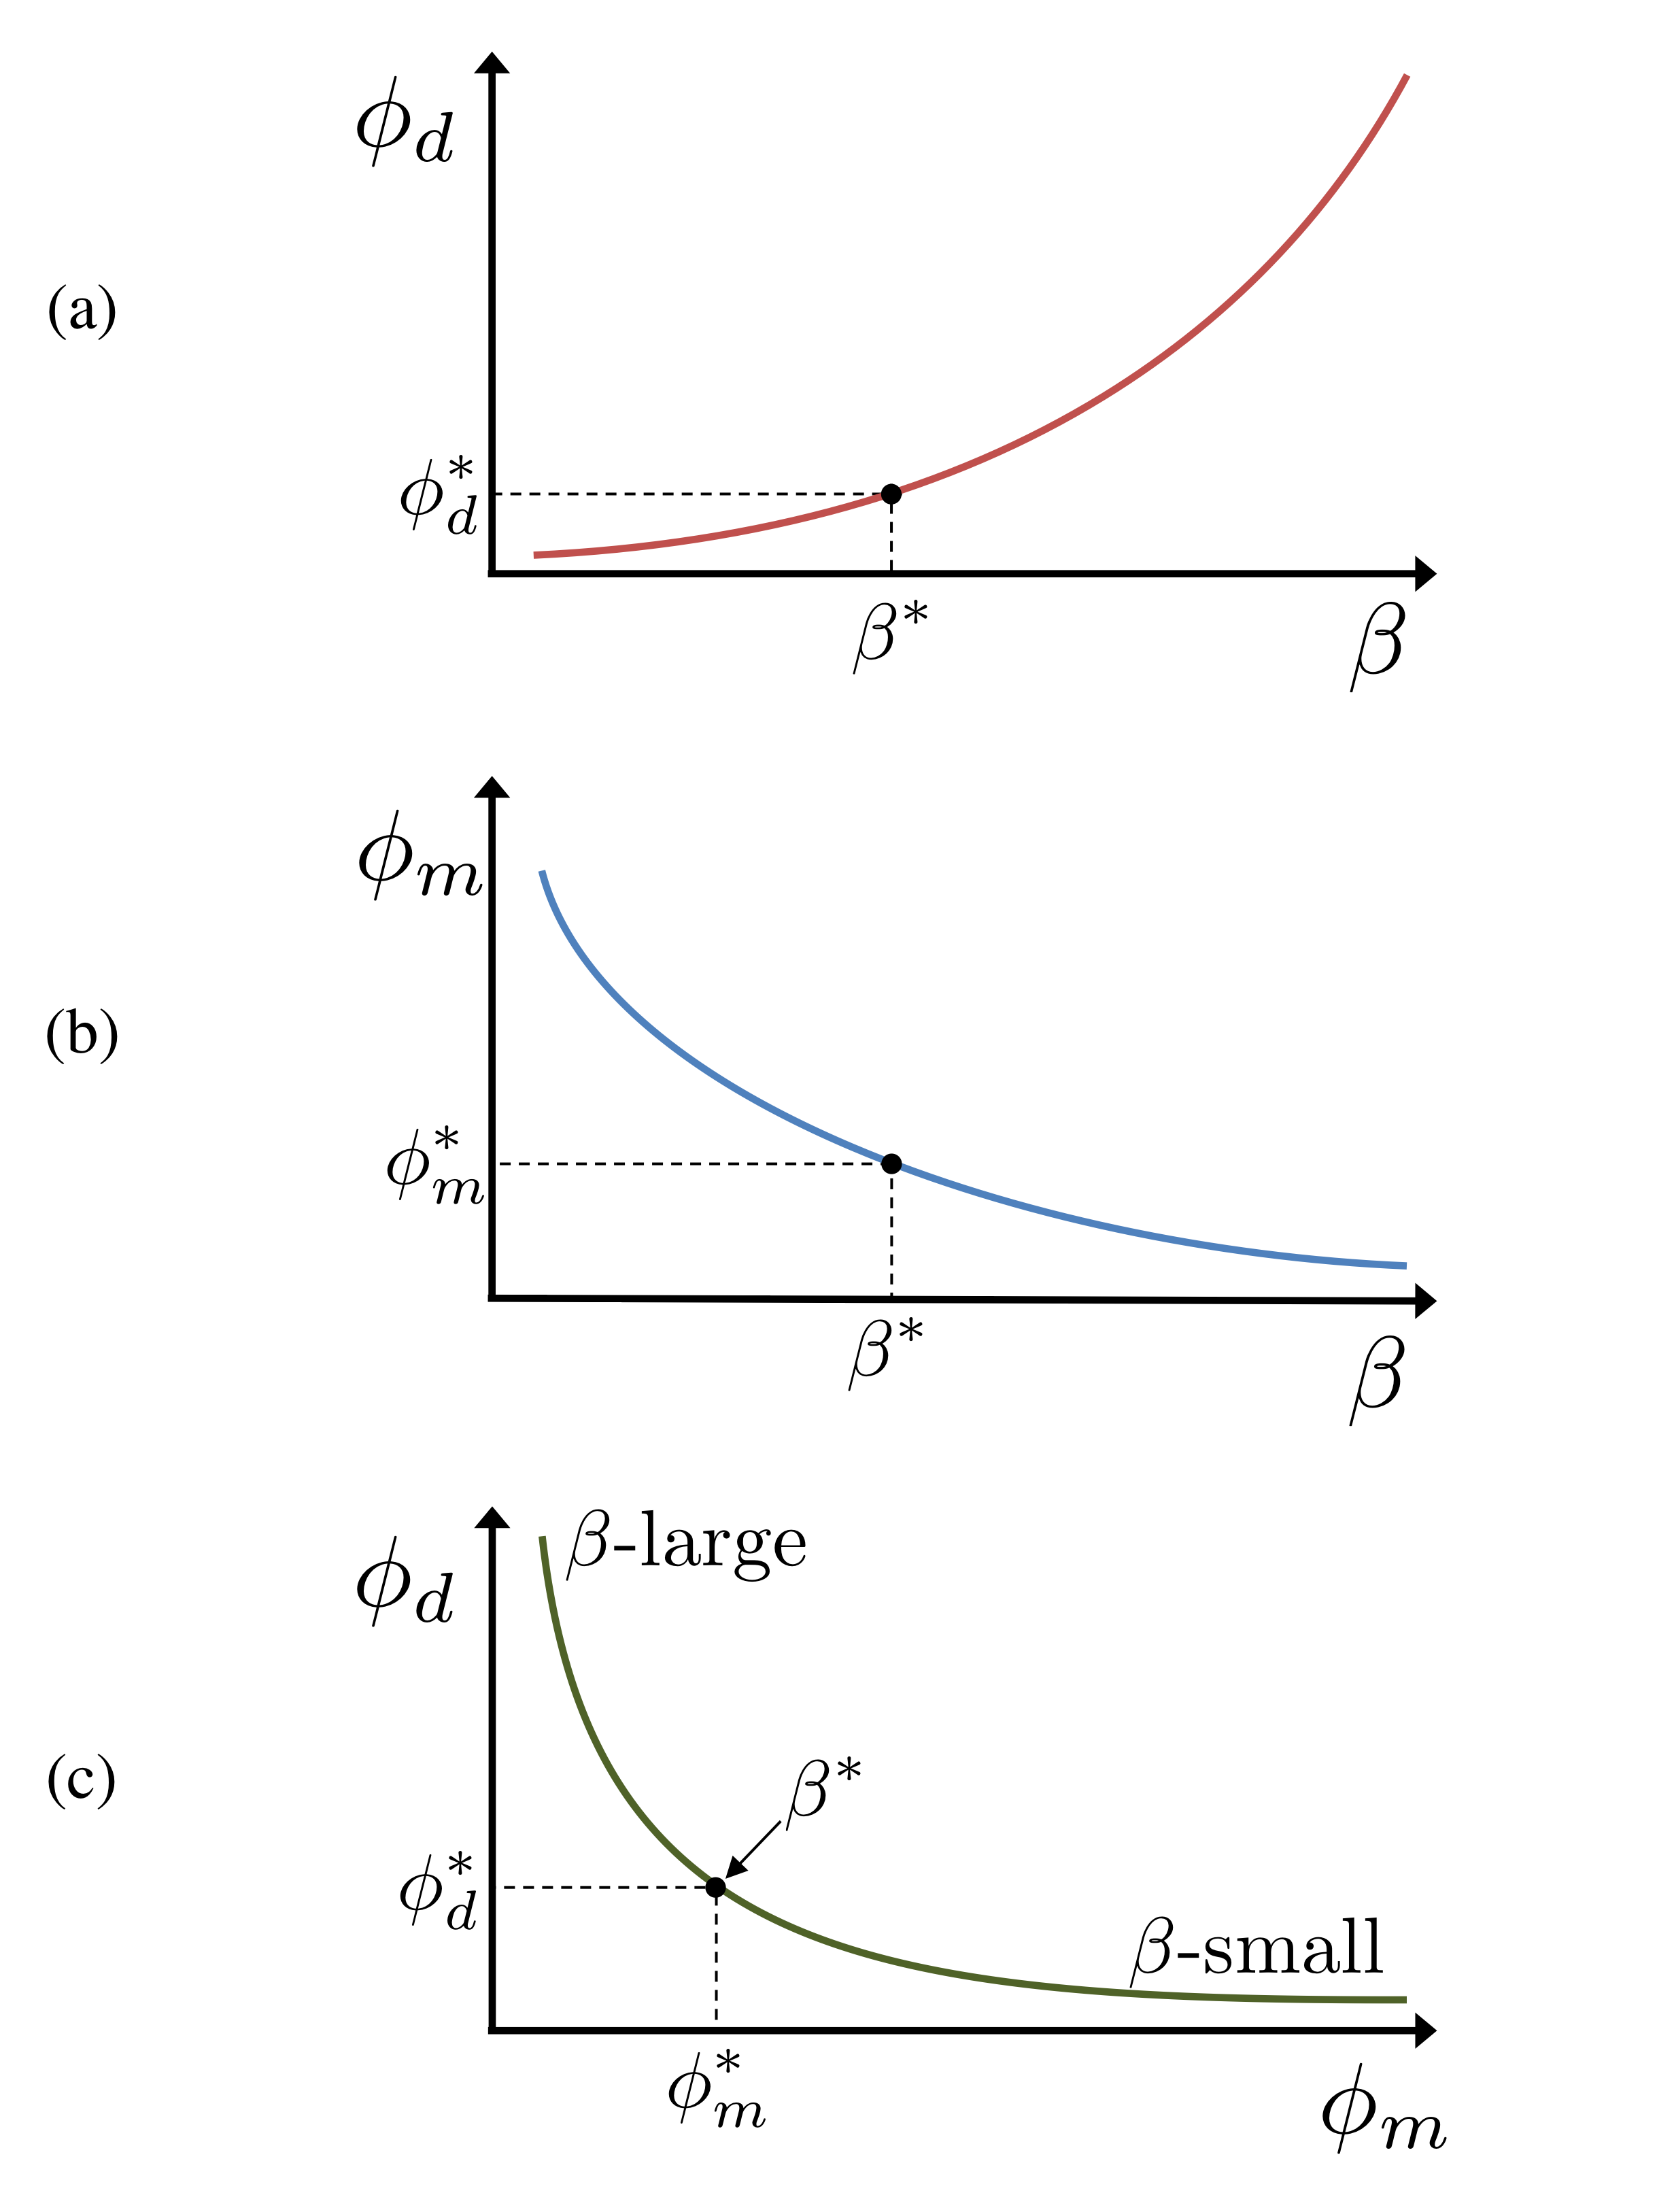
\includegraphics[width=7.5cm]{images/betafig.png}
% \caption{(a) Data misfit vs. $\beta$, (b) regularization vs. $\beta$, (c) Tikhonov curve}
% \label{fig:TradeOffs}
% \end{figure}
An optimum value, $\beta^*$, can be found
so that minimizing equation \ref{eq:Phi} with $\beta^*$ produces a model with misfit $\phi_d^*$. The
value of $\beta^*$ can be found via cooling techniques where the $\beta$ is progressively
reduced from some high value and the process stopped when the tolerance is reached, or using
two-stage methods as advocated by {\cite{Parker1977}}.
There are other strategies for selecting the trade-off parameter including:
the L-curve technique \citep{hansen1992analysis}, which attempts to find the point of greatest curvature in the Tikhonov curve;
and Generalized Cross Validation \citep{wahba1990spline,golub1979generalized,golub1997generalized,haber2000gcv,DougTutorial,Farquharson2004}.

The optimization posed in equation \ref{eq:invoptimization} is almost always non-linear.
It is linear only in the special case that the forward mapping is a linear functional
of the model, $\phi_m$ and $\phi_d$ are written as $l_2$ norms, $\beta$ is known, and that there are no
imposed bound constraints. This rarely happens in practice, requiring that iterative optimization methods be employed to find a solution.
Gradient-based methods are commonly used and the reader is referred to \cite{Nocedal1999},
for background and introductions to the relevant literature. For geophysical problems,
Gauss-Newton techniques have proven to be valuable and practical. For $l_2$ norms we
write the objective function as
{%\iftoggle{finaldraft}{
\begin{equation}
\phi(\m) = \frac{1}{2}||\Wd(F[\m]-\dobs)||^2_2 + \frac{1}{2} \beta ||\Wm(\m-\mref)||^2_2.
\end{equation}
}
The gradient is given by
{%\iftoggle{finaldraft}{
\begin{equation}
g(\m)= J[\m]^\top \Wd^\top \Wd(F[\m]-\dobs) + \beta \Wm^\top \Wm (\m-\mref),
\end{equation}
}
where $J[\m]$ is the sensitivity or Jacobian. The components $J[\mathbf{m}]_{ij}$ specify how the $i$\textsuperscript{th} datum
changes with respect to the $j$\textsuperscript{th} model parameter; this will be discussed in more detail in the next section. At the $k$\textsuperscript{th} iteration, beginning with a model $\m^{k}$,
we search for a perturbation $\delta \m$ that reduces the objective function.
Linearizing the forward simulation by
{%\iftoggle{finaldraft}{
\begin{equation}
F[\m^{k}+\delta \m] \approx F[\m^{k}] + J[\m^{k}]\delta \m %+ \mathcal{O}(\delta m)^2
\end{equation}
}
and setting the gradient equal to zero yields the standard Gauss-Newton equations
to be solved for the perturbation $\delta \m$:
{%\iftoggle{finaldraft}{
\begin{equation}
\label{eq:gn}
 (J[\m]^\top \Wd^\top \Wd J[\m] + \beta \Wm^\top \Wm) \delta \m = -g(\m).
\end{equation}
}
The updated model is given by
{%\iftoggle{finaldraft}{
\begin{equation}
\m^{k+1}=\m^{k} + \gamma \delta \m,
\end{equation}
}
where $\gamma \in (0,1]$ is a coefficient that can be found by a line search.
Setting $\gamma=1$ is the default and a line search is necessary if
$\phi(\m^{k+1}) \ge \phi(\m^{k})$.

The iterative optimization process is continued until a suitable stopping criterion is reached.
Completion of this iterative process yields a minimization for particular value
of the trade-off parameter, $\beta$. If we are invoking a cooling schedule, and if the
desired misfit tolerance is not yet achieved, $\beta$ is reduced
and the iterative numerical optimization procedure is repeated. % to clarify that iterative is referring to the optimization machinery

\subsubsection*{Sensitivities}

A central element in the above approach is the computation of the sensitivities.
The sensitivity functional is defined by
{%\iftoggle{finaldraft}{
\begin{equation}
J[\mathbf{m}] = \deriv{F[\m]}{\m} = \mathbf{P}\left(\deriv{\u}{\m}\right),
\label{eq:J}
\end{equation}
}
where $\bf P$ is a linear projection, and $d\cdot$ indicates total difference.
There are numerous approaches to computing the sensitivity but the chosen methodologies are dictated by the size of the problem.
The discrete sensitivity matrix, $\bf J$, is a dense $N \times M$ matrix, where $N$ is the number
of data and $M$ is the number of model parameters. For some problems, $\bf J$
can be computed directly and stored. Ultimately this demands the solution of
numerous forward problems (cf. \cite{haber2015computational}). Another approach is to factor $J[\mathbf{m}]$ in symbolic
form.
In the general case, we solve for the sensitivity implicitly by taking the derivative of $C(\m,\u)=0$ (equation \ref{eq:fwdmodel}) to yield:

% DWO: not keen on this notation; A(m)u=q
{%\iftoggle{finaldraft}{
\begin{equation}
\label{eq:dcdm_dcdu}
    \nabla_\m C(\m,\u) d \m  +
    \nabla_\u C(\m,\u) d \u
    = 0,
\end{equation}
}
where $\nabla_{\cdot}$ indicates partial difference, and both $\nabla_\m C(\m,\u)$ and $\nabla_\u C(\m,\u)$ are matrices.
For a given model, $\nabla_\u C(\m,\u)$ corresponds to the forward simulation operator, and if the forward problem is well-posed, then the matrix is invertible \citep{haber2015computational}.
Equation~\ref{eq:dcdm_dcdu} can be rearranged to
{%\iftoggle{finaldraft}{
\begin{equation}
\label{eq:dcdm_dcdu_rearranged}
d \u =
    - \left(\nabla_\u C(\m,\u)\right)^{-1}
    \nabla_\m C(\m,\u) d \m,
\end{equation}
}
and combined with equation~\ref{eq:J} to obtain a formula for the sensitivity matrix.
We note that this matrix is dense, often large, and need not actually be formed and stored.



\subsubsection*{Inversion as optimization}


%%%%%%%%%%%%%%%%%%%%%%%%%%%%%%%%%%%%
%%%%   Numerical Optimization   %%%%
%%%%%%%%%%%%%%%%%%%%%%%%%%%%%%%%%%%%
Once the inverse problem has been stated in an optimization framework (equation \ref{eq:invoptimization}),
an appropriate optimization routine can be selected.
For example, if bound constrains are incorporated, a projected Gauss-Newton algorithm can be used.
In large-scale inversions, special attention may have to be given to ensuring a memory efficient
optimization algorithm, however, the underlying mechanics of the algorithms often remain unchanged. % something like that.
In a geophysical inversion we require a model that is consistent with \emph{a priori} information and
known or assumed statistical distributions. % e.g. the Discrepancy Principle.
As such, the stopping criteria of the inversion are often implemented differently than traditional optimization algorithms,
or a series of incomplete optimization algorithms are invoked while changing the objective function \citep{DougTutorial,haber2015computational,haber2000optimization}.
%As such, the optimization algorithm must have a way of `warm-starting' if it is to be computationally efficient.

%%%%%%%%%%%%%%%%%%%%%%%%%%%%%%%%%%%%
%%%%%%%%%%    Inversion   %%%%%%%%%%
%%%%%%%%%%%%%%%%%%%%%%%%%%%%%%%%%%%%
% We define the geophysical inversion as the whole process by which
% a geophysicist creates a preferred model (or set of models).
The optimization of the stated inverse problem
provides the machinery to obtain a mathematical solution. However, before the model is
accepted as a viable candidate, there are numerous questions that
should be investigated.
For example, questions to be addressed might include:
(a) How well does the recovered model fit the observed data?
(b) Is there bias in the misfits between the observed and predicted data?
(c) What was the path for the convergence?
(d) Is there too much or too little structure?
(e) Does the model fit with prior knowledge and other data sets?
% (f) What was the Tikhonov curve?
The final results and details about
how the inversion algorithm has performed all provide clues as
to whether the constructed model can be accepted, or if elements in
our procedure or its numerical implementation need to be altered and
the inversion rerun. This might include adjusting the assigned
uncertainties in the misfit function, altering the model regularization, or changing aspects of the numerical computations.


\subsection{Evaluation/Interpretation}

In this section we return to the initial question posed for which the inversion
was designed to help answer.
Items of interest might include:
(a) Are the interesting features supported by the data or are they artifacts?
(b) Does the result make sense geologically and geophysically?
(c) Are there interesting features that should be investigated further? %Existence of features or structures.
Addressing these questions usually involves repeating the inversion process
with appropriate modifications (cf. \cite{DougTutorial,Pidlisecky2011,lines1988cooperative}).
As such, we require an implementation that is inherently and unequivocally modular,
with all pieces available to manipulation.
Black-box software, where the
implementations are hidden, obfuscated, or difficult to manipulate,
do not promote experimentation and investigation.
Exposing the details of the implementation to the geophysicist in
a manner that promotes productivity and question-based interrogation
is the goal of \SimPEG and is the topic of the next section.


%%%%%%%%%%%%%%%%%%%%%%%%%%%%%%%%%%%%
%%%%%% MODULAR IMPLEMENTATION %%%%%%
%%%%%%%%%%%%%%%%%%%%%%%%%%%%%%%%%%%%

\section{Modular Implementation}
\label{sec:implementation}

There are an overwhelming amount of choices to be made as one works through the forward
modeling and inversion process (Figure~\ref{fig:inversionOutline}). As a result,
software implementations of this workflow often become
complex and highly interdependent, making it difficult to interact with and to
ask other scientists to pick up and change.
Our approach to handling this complexity is to propose a framework,
Figure~\ref{fig:classOutline}, that compartmentalizes the implementation of
inversions into various units.
We present it in this specific modular style, as each unit contains
a targeted subset of choices crucial to the inversion process.

The aim of the \SimPEG framework and implementation
is to
allow users to move between terminology, math, documentation and
code with ease, such that there is potential for development in a scalable way.
The \SimPEG implementation provides a library that mimics the framework shown in Figure~\ref{fig:classOutline} with each unit representing a base class.
These base classes can be inherited in specific geophysical problems to accelerate development
as well as to create code that is consistent between geophysical applications.


% \begin{itemize}
%     \item want dissemination of this package.
%     \item no compiling required
%     \item Geared towards the inverse problem
%     \item The framework is malleable into different workflows, e.g. synthetic
%         data vs. real data forward simulation vs inverse modeling
%     \item Framework has been designed with forethought for interactivity and modularity.
% \end{itemize}

\subsection{Implementation Choices}
We chose Python \citep{python} for the implementation
of \SimPEG. Python supports object-oriented practices, interactive
coding, has extensive support for documentation, and has a large and
growing open source scientific community \citep{Lin2012}.
% As an interpreted language, there are occasionally bottlenecks on speed or
% memory. These inefficiencies may mean that the code will not be able to
% scale to a production quality code. However, these computational
% bottlenecks can often be identified through profiling and can be written
% in a lower-level language and wrapped in Python.
% Additionally, these problems are admissible when the goal of the software
% is clear: we require an interactive research tool where geophysical
% problems from many disciplines live in one place to enhance
% experimentation and dissemination of new ideas.
To enhance the dissemination of our work, we have released our work under
the permissive MIT license for open source software.
The MIT License does not force packages that use \SimPEG to be open source
nor does it restrict commercial use. We have also ensured
that our practices with regard to version control, code-testing and documentation follow
best practices \citep{Wilson2014}.

\subsection{Overview}
As discussed in the previous section, the process of obtaining an acceptable model
from an inversion generally requires the geophysicist to perform several iterations
of the inversion workflow, rethinking and redesigning each piece of the framework to
ensure it is appropriate in the current context.
Inversions are experimental and empirical by nature and our software package is designed to facilitate this iterative process.
% For a software package to be useful, this iterative process must be efficient from the \emph{researcher's}
% point of view, as inversions are experimental and empirical by nature.
To accomplish this, we have divided the inversion methodology into eight major
components (Figure~\ref{fig:classOutline}).
The \Mesh class handles the discretization of the earth and
also provides numerical operators. The forward simulation is split into two
classes, the \Survey and the \Problem. The \Survey class handles the geometry
of a geophysical problem as well as sources. The \Problem class handles the simulation of the physics for
the geophysical problem of interest. Although created independently, these
two classes must be \emph{paired} to form all of the components necessary for a
geophysical forward simulation and calculation of the sensitivity.
The \Problem creates geophysical fields given a source from the \Survey.
The \Survey interpolates these fields to the receiver locations and converts them to the appropriate data type, for example, by selecting only the measured components of the field.
% projects these computed fields onto the data space at the receiver locations. %type and location
Each of these operations may have associated derivatives with respect to the model and the computed field; these are included in the calculation of the sensitivity.
For the inversion, a \DataMisfit is chosen to capture the \emph{goodness of fit} of the predicted data and a \Regularization is chosen to handle the non-uniqueness.
These inversion elements and an \Optimization routine are combined into an inverse problem class (\InvProblem).
\InvProblem is the mathematical statement (i.e. similar to equation~\ref{eq:invoptimization})
that will be numerically solved by running an \Inversion. The \Inversion
class handles organization and dispatch of \emph{directives} between all
of the various pieces of the framework.

{%\iftoggle{finaldraft}{
\begin{figure}[ht!]
\centering
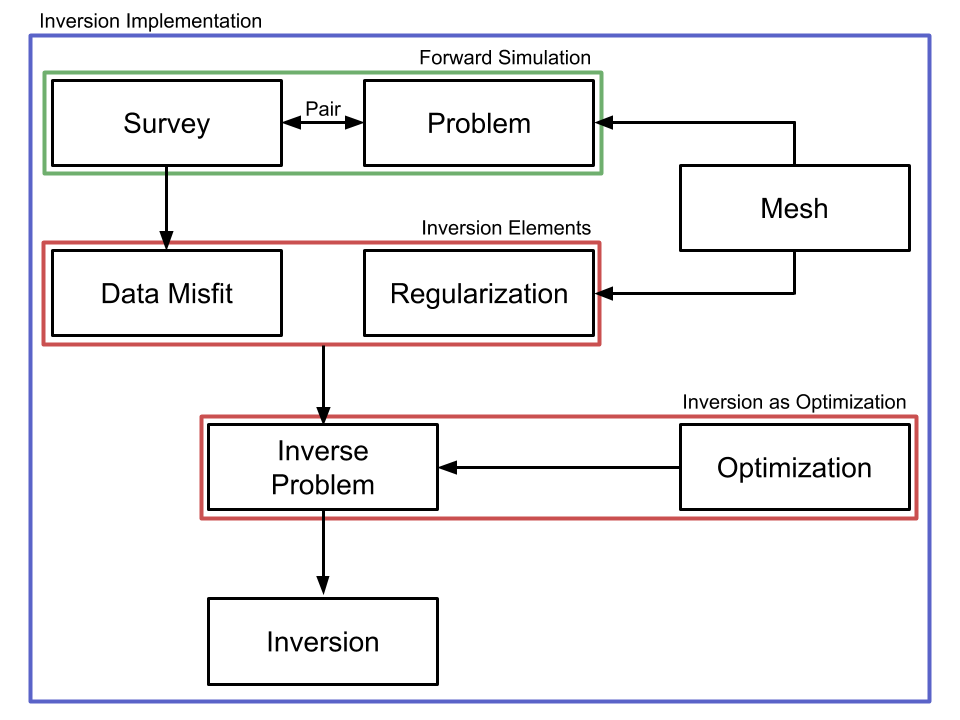
\includegraphics[width=7.5cm]{images/SimPEGFrameworkRevised.png}
\caption{\SimPEG framework indicating the flow of information. In the implementation, each of these modules is a base class.}
%Overview of classes that implement the modular \SimPEG framework.}
\label{fig:classOutline}
\end{figure}
}

The arrows in the Figure~\ref{fig:classOutline} indicate what each class
takes as a primary argument. For example, both the \Problem and \Regularization
classes take a \Mesh class as an argument. The diagram
does not show class inheritance, as each of the base classes outlined have
many subtypes that can be interchanged. The \Mesh class, for example, could
be a regular Cartesian mesh or a cylindrical coordinate mesh, which have
many properties in common. These common features, such as both meshes
being created from tensor products, can be exploited through inheritance
of base classes, and differences can be expressed through subtype
polymorphism. We refer the reader to the online, up-to-date documentation (http://docs.simpeg.xyz) to look at the class inheritance structure in depth.

\subsection{Motivating Example}
\label{sub:motivating_example}
We will use the DC resistivity problem from geophysics
to motivate and explain the various components of the \SimPEG framework. This example will be
referred to throughout this section; we will introduce it briefly here,
and refer the reader to \cite{Pidlisecky2007} %{\color{red}CITE DOUG question??}
for a more in-depth discussion.
The governing equations for DC resistivity are:
{%\iftoggle{finaldraft}{
\begin{equation}
\label{eq:dc}
\nabla \cdot ( - \sigma \nabla \phi) = I(\delta(\vec{r}-\vec{r}_{s^+}) - \delta(\vec{r}-\vec{r}_{s^-})).
\end{equation}
}
Where $\sigma$ is the electrical conductivity,
$\phi$ is the electric potential,
$I$ is the input current at the positive and negative dipole locations $\vec{r}_{s^\pm}$, captured as Dirac delta functions.
In DC resistivity surveys, differences in the potential field, $\phi$, are sampled using dipole receivers to collect observed data.
To simulate this partial differential equation (PDE) (or set of PDEs, if there are multiple current injection locations), we must discretize the equation onto a computational mesh.

\subsection{Mesh}
\label{sub:mesh}

Any numerical implementation requires the discretization of continuous
functions into discrete approximations. These approximations are typically
organized in a mesh, which defines boundaries, locations, and
connectivity. Of specific interest to geophysical simulations, we require
that averaging, interpolation and differential operators be defined for
any mesh. In \SimPEG, we have implemented a staggered mimetic finite
volume approach \citep{Hyman1999,Hyman2002}. This approach requires the definitions of
variables at either cell-centers, nodes, faces, or edges as described in
Figure~\ref{fig:meshLocations}. We will focus our attention on explaining
our implementation of a tensor mesh. A more detailed explanation can be
found in \cite{haber2015computational}.
To create a new \Mesh instance, a \texttt{TensorMesh} class can be selected from the
\SimPEG Mesh module and instantiated with a list of vectors:

{%\iftoggle{finaldraft}{
% \begin{minted}[tabsize=4,mathescape,
%                numbersep=5pt,
%                framesep=2mm,
%                fontsize=\scriptsize]{python}
{\scriptsize\begin{verbatim}
    from SimPEG import Mesh, Solver, Utils, np, sp
    hx = np.ones(30)
    hy = np.ones(30)
    mesh = Mesh.TensorMesh([hx,hy])
\end{verbatim}}
% \end{minted}
}
\noindent
Here, the \SimPEG library is imported, as well as NumPy (\texttt{np}) and SciPy's sparse
matrix package (\texttt{sp}) \citep{scipyOliphant,scipy}. The vectors \texttt{hx} and \texttt{hy} describe the cell size in each mesh dimension. The dimension of the mesh is defined by the length of the list, requiring very little change to switch mesh dimensions or type.
Once an instance of a mesh is created, access to the properties and methods shown in
Table~\ref{table:Mesh} is possible. There are additional methods and visualization routines that are also included in the \SimPEG \Mesh classes.
Of note in Table~\ref{table:Mesh} are
organizational properties (such as counting, and geometric properties),
locations of mesh variables as Cartesian grids,
differential and averaging operators,
and interpolation matrices.
The mesh implementation can be readily extended to
other types of finite volume meshes, for example, OcTree \citep{HaHe06}, logically
rectangular non-orthogonal meshes \citep{Hyman2002}, and unstructured meshes \citep{Ollivier-gooch2002}.
Additionally, this piece of the framework
may be replaced by other methodologies such as finite elements.
% These extensions and substitutions are often very advantageous in
% certain situations, however, they will not be the focus of this discussion.

{%\iftoggle{finaldraft}{
\begin{figure}[ht!]
\centering
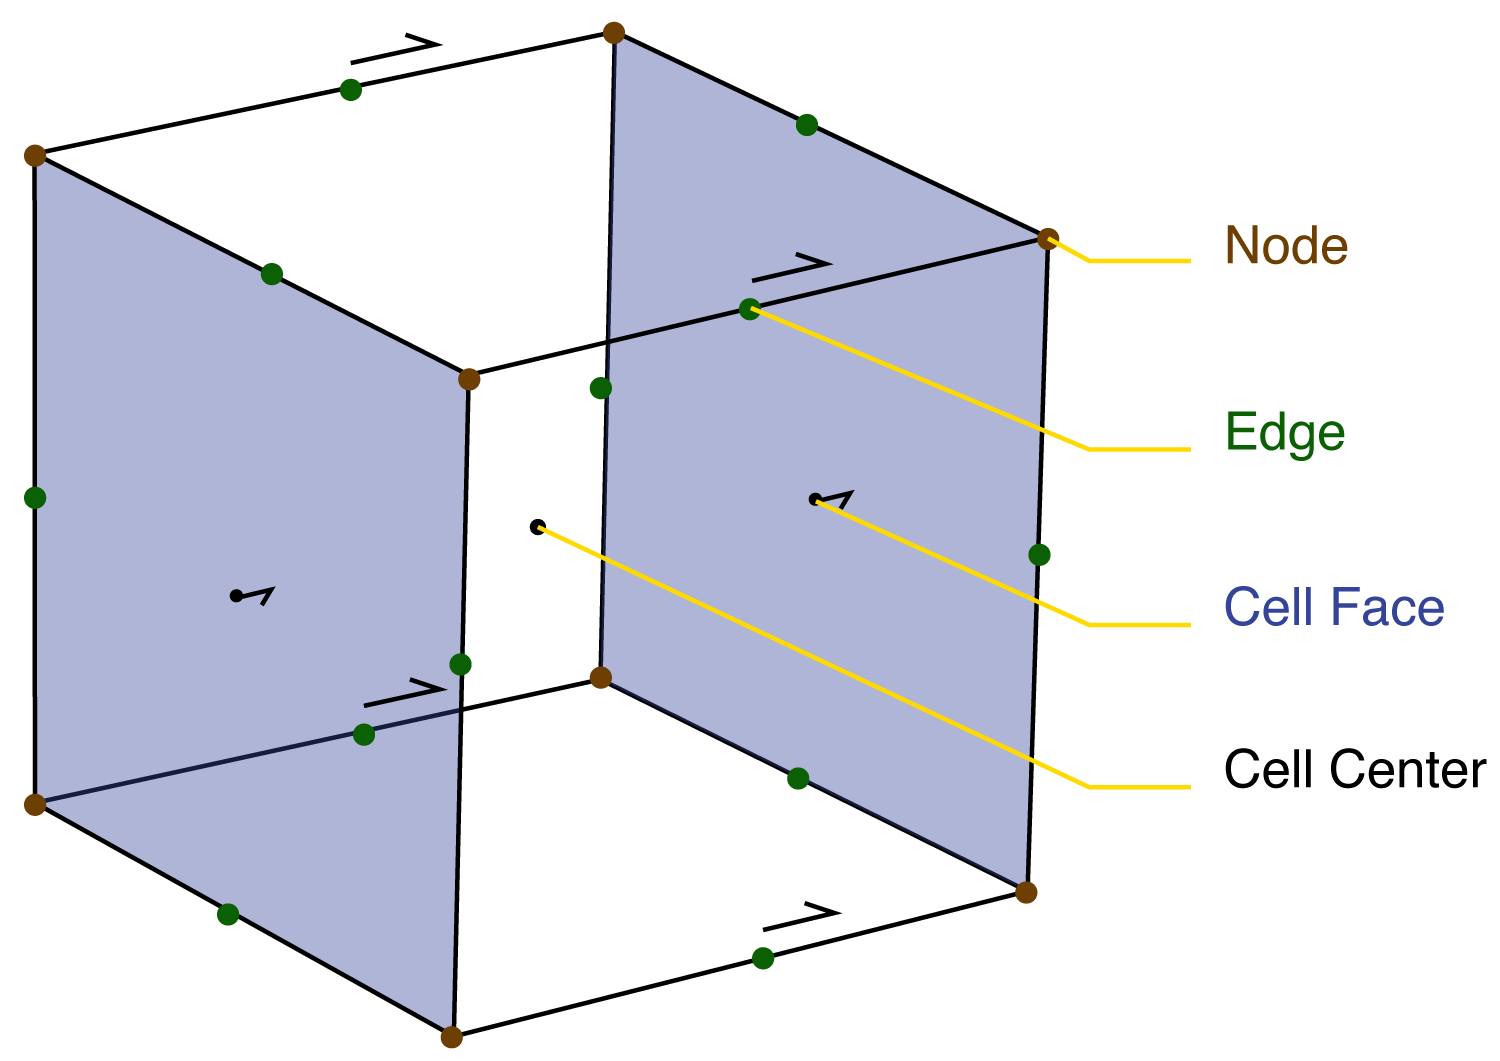
\includegraphics[width=7.5cm]{images/cube.png}
\caption{Location of variable in a single voxel of a three dimensional finite volume discretization.}
\label{fig:meshLocations}
\end{figure}
}

{%\iftoggle{finaldraft}{
\begin{table}[ht]
\caption{Selected \Mesh class properties with explanations.}
\scriptsize
\label{table:Mesh}
  \begin{tabular}{  p{2.5cm}  p{4.5cm} }
    \hline

    Property or Function & Explanation \\ \hline
    dim  & Dimension of the mesh\\
    x0  & Location of the origin\\
    nC, nN, nF, nE & The number of cells, nodes, faces, or edges. (e.g. nC is the total number of cells)\\
    % vnC, vnN, vnF, vnE & Number of cells as vectors (e.g. \texttt{vnC == [nCx, nCy, nCz]})\\
    vol, area, edge  & Geometric measurements for the mesh\\ % (w.r.t. 3D nomenclature)
    gridN, gridCC, etc.  & Array of grid locations\\
    nodalGrad  &  Gradient of a nodal variable $\rightarrow$ edge variable\\
    faceDiv  & Divergence of a face variable $\rightarrow$ cell-centered variable\\
    edgeCurl  & Curl of a edge variable $\rightarrow$ face variable\\
    cellGrad  & Gradient of a cell-centered variable $\rightarrow$ face variable\\
    aveF2CC, aveN2CC, etc.  & Averaging operators (e.g. F$\rightarrow$CC, takes values on faces and averages them to cell-centers)\\
    % getEdgeInnerProduct(), getFaceInnerProduct()  & Inner product operators for material properties\\
    getInterpolationMat(loc)  & Interpolation matrix for xyz locations\\

    \hline
  \end{tabular}
\end{table}
}

% The differential operators for the meshes under consideration are
% created using the geometrical definitions of the gradient, divergence,
% and curl (cf. \cite{Hyman1999}) leading to a mimetic discretization.
% For example, the divergence of a flux $\vec{J}$ can be formally written as:
% {%\iftoggle{finaldraft}{
% \begin{equation}
% \text{div}\vec{J} =  \lim_{V \rightarrow 0}
% \iint_{S(V)} \frac{\vec{J}\cdot\vec{n} }{ |V| } dS
% \end{equation}
% }
% Here the discretization is relatively simple:
% {%\iftoggle{finaldraft}{
% {\scriptsize\begin{verbatim}
%     S = mesh.area
%     V = mesh.vol
%     faceDiv = sdiag(1/V)*D*sdiag(S)
% \end{verbatim}}
% }
% \noindent
% Where \texttt{sdiag} puts an array on the diagonal of a sparse matrix; and
% \texttt{D} is a stencil matrix of $\pm 1$ that indicates fluxes into or out of a
% cell. This stencil is constructed efficiently for
% a tensor mesh using kronecker products \citep{haber2015computational}. Here we note that
% our conventions for referring to areas, edge lengths, and volumes
% are with regard to a 3D mesh, however, the nomenclature used for
% 1D and 2D remain the same. As such, the length of the `volume'
% array is always equal to the number of cells in the mesh:
% {%\iftoggle{finaldraft}{
% {\scriptsize\begin{verbatim}
%     len(mesh.vol)  == mesh.nC
%     len(mesh.area) == mesh.nF
%     len(mesh.edge) == mesh.nE
% \end{verbatim}}
% }

The \Mesh interface allows for lazy loading of properties, that is,
all properties of the mesh are created on demand and then stored for
later use. This is important as not all operators are useful in all
problems and, as such, are not created. The implementation here is different
from some other finite volume implementations as the operators are held
in memory as matrices and are readily available for interrogation.
We find this feature to be extremely beneficial for educational
and research purposes as the discretization remains visually very
close to the math, and the matrices can be manipulated,
visually inspected, and combined readily.

With the differential operators readily accessible, simulation of a cell-centered
discretization for conductivity, $\sigma$, in the DC resistivity problem is straight-forward.
The discretized system of equation \ref{eq:dc} can be written as
{%\iftoggle{finaldraft}{
\begin{equation}
    \bf A(\sigma) \u = D (M_{1/\sigma}^f)^{-1} G \u = - q,
\end{equation}
}
where $\bf D$ and $\bf G$ are the divergence and gradient operators, respectively. The conductivity, $\sigma$, is harmonically averaged from cell-centers to cell-faces to create the matrix $\bf (M_{1/\sigma}^f)^{-1}$ \citep{Pidlisecky2007}. In \SimPEG this is written as:
{%\iftoggle{finaldraft}{
{\scriptsize\begin{verbatim}
    D = mesh.faceDiv
    G = mesh.cellGrad
    Msig = Utils.sdiag(1/(self.mesh.aveF2CC.T * (1/sigma)))
    A = D*Msig*G
\end{verbatim}}
}
The code is easy to read, looks similar to the math, can be built interactively
using tools such as IPython \citep{Perez2007}, and is not dependent on the dimension of mesh used. Additionally, it is decoupled from the mesh type, for example Figure \ref{fig:threeMeshes} is generated by solving a \texttt{DCProblem} for three different mesh types: \texttt{TensorMesh}, \texttt{TreeMesh} and \texttt{CurvilinearMesh}. Other than the specific mesh generation code, no other modifications to the DC problem were necessary (see the online examples provided in \SimPEG).
Given the electrode locations, a $\bf q$ can be constructed on each mesh and the system
$\bf A(\sigma) \u = - q$
solved.
\SimPEG comes with a few different types of \texttt{Solver} objects that provide
a simple and common interface to direct and iterative solvers found across many different Python packages.
{%\iftoggle{finaldraft}{
{\scriptsize\begin{verbatim}
    Ainv = Solver(A) # Create a solver object
    u = Ainv * ( - q )
    mesh.plotImage(u)
\end{verbatim}}
}
The potential field can be projected onto the receiver electrode locations
through interpolation matrices constructed by the \Mesh class.
Additionally, there are multiple visualization routines that have
been included in the \Mesh class for rapid visualization and
interrogation of geophysical fields and physical properties (Figure \ref{fig:threeMeshes}).
We note that these code snippets can be easily be combined in a script, highlighting the
versatility and accessibility of the \Mesh classes in \SimPEG.

{%\iftoggle{finaldraft}{
\begin{figure}[ht!]
\centering
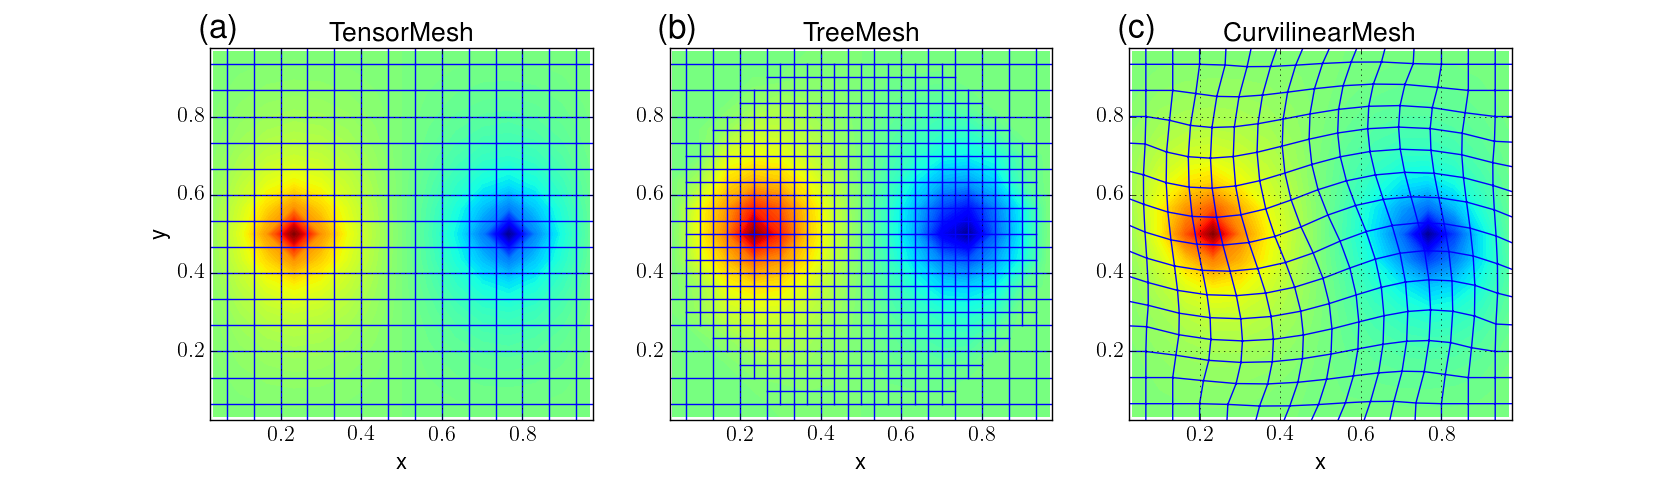
\includegraphics[width=15.5cm]{images/ThreeMesh.png}
\caption{Solving the DC resistivity problem for a dipole and using the meshes visualization routine for the potential,
$\phi$, for three different mesh types: (a) TensorMesh, (b) TreeMesh, and (c) CurvilinearMesh. The potential has been interpolated onto the tensor mesh for visualization.}
\label{fig:threeMeshes}
\end{figure}
}

This script will be expanded upon and segmented into the various pieces of
the framework in the following sections. We find that the development of
geophysical codes is often iterative and requires `scripting' of equations.
Only after these are correct, as demonstrated by an appropriate test (e.g. \texttt{Tests.checkDerivative}), do we formalize and segment our script to enable a geophysical
inversion to be run. The toolbox that \SimPEG provides promotes this interactive and
iterative style of development.


\subsection{Forward simulation}

The forward simulation in \SimPEG is broken up into a \Survey class and
a \Problem class.
The \Problem class contains the information and code that capture the physics
used to describe the connection between a physical property distribution and the
fields/fluxes that are measured in a geophysical survey.
The \Survey class contains information about the observed data and
the geometry of how to collect the data (e.g. locations and types of receivers
and sources) given a \Problem that simulates fields. The \Problem
and the \Survey must be \emph{paired} together to simulate predicted data.
We decided on this separation of the code because it is possible to have
multiple mathematical descriptions, of varying complexities, that explain the same
observed data. For example, a seismic simulation could have multiple approximations
to the physics which increase in complexity and accuracy, from straight-ray tomography, Eikonal tomography,
to full waveform simulation. Additionally, there are often multiple types
of geophysical surveys that could be simulated from the same \Problem class.

{%\iftoggle{finaldraft}{
\begin{table}[ht]
\caption{Base \Problem class properties with explanations.}
\scriptsize
\label{table:Problem}
  \begin{tabular}{  p{2.5cm}  p{4.5cm} }
    \hline

    Property or Function & Explanation \\ \hline

    fields(m)   & Calculation of the fields given a model\\
    Jvec(m, v)  & Sensitivity times a vector\\
    Jtvec(m, v) & Adjoint sensitivity times a vector\\
    % Jfull(m)    & Full sensitivity matrix\\
    mapping     & Maps the model to a physical property\\

    \hline
  \end{tabular}
\end{table}
}


The crucial aspects of the \Problem class are shown in Table~\ref{table:Problem},
and the properties and methods of the \Survey class are shown in Table~\ref{table:Survey}.
We note that each of the sub-classes of \Problem will implement fields and
sensitivities in a different way, likely with additional methods and properties.
Furthermore, the choice of terminology becomes clearer when these
classes are inherited and used in a specific geophysical method (e.g. a \DCProblem or \EMProblem).
For the \DCProblem, the \texttt{fields} can be created by constructing $\mathbf{A(m)}$
and solving with the source terms, $\mathbf{Q}$,
which will be provided by the \DCSurvey's source list (\texttt{srcList}).
Each source has at least one receiver associated with it;
the receivers can create a matrix, $\mathbf{P}$, that project the
fields, $\u$, onto the data-space. For example, in the DC problem, a dipole receiver samples the potential at each electrode location and computes the difference to give a datum.
We note that the process of computing a datum may be more involved and have derivatives with respect the computed fields and possibly the model.
Much of the organizational
bottlenecks are taken care of through general receiver and source classes,
which can be inherited and tailored to the specific application.
The \texttt{mapping} in the \Problem provides a transform from an arbitrary model to a discretized grid function
of physical properties. For example, log-conductivity is often used in the
inverse problem for DC resistivity rather than parameterizing
directly in terms of conductivity. If this choice is made for the model,
an appropriate map (i.e. the exponential) must be provided to transform from the model space to the
physical property space (cf. \cite{HeagySEG2014}).

{%\iftoggle{finaldraft}{
\begin{table}[ht]
\caption{Selected \Survey class properties with explanations.}
\scriptsize
\label{table:Survey}
  \begin{tabular}{  p{2.5cm}  p{4.5cm} }
    \hline

    Property or Function  & Explanation \\ \hline

    dobs, nD                 & $\dobs$, number of data\\
    std                      & Estimated standard deviations\\
    srcList                   & List of sources with associated receivers\\
    dpred(m)                 & Predicted data given a model, $\dpred(m)$\\
    projectFields(m, u)      & Projects the fields, $P(m,u)$\\
    projectFieldsDeriv(m, u) & Derivative of the projection, $\deriv{P(m,u)}{m}$\\
    residual(m)              & $\dpred(m) - \dobs$\\

    \hline
  \end{tabular}
\end{table}
}

\subsection{DC resistivity forward simulation}
\label{sec:DCforward}

A simple DC-resistivity survey is presented to demonstrate some of the components of \SimPEG in action.
A set of Schlumberger arrays is used to complete a vertical sounding.
In this example, we have taken our scripts from the previous section describing the forward simulation
and combined them in a package called \texttt{simpegDC} (http://simpeg.xyz).
We use the 3D tensor \texttt{mesh} to run the forward simulation for the data of this problem.
{%\iftoggle{finaldraft}{
{\scriptsize\begin{verbatim}
    import simpegDC as DC
    survey = DC.SurveyDC(srcList)
    problem = DC.ProblemDC(mesh)
    problem.pair(survey)
    data = survey.dpred(sigma)
\end{verbatim}}
}
\noindent
Here the \texttt{srcList} is a list of dipole sources (\texttt{DC.SrcDipole}),
each of which contains a single receiver (\texttt{DC.RxDipole}). %get potentials and computes a difference
Similar to the illustration in Figure~\ref{fig:classOutline}, the \Problem and the \Survey must be paired for either
to be used to simulate fields and/or data.
% Computed responses from a homogeneous half-space with a resistivity of 100 $\Omega$m converted to apparent resistivity as shown in Figure \ref{fig:DCfwd}(b) using:
% \begin{equation}
%     \rho_a = \frac{V}{I}\pi\frac{b(b+a)}{a},
% \end{equation}
% where $a$ and $b$ are the separations between MN (potential) and AB (current) electrodes, respectively. The computed apparent resistivities show a reasonable match with analytic responses as shown in Figure ~\ref{fig:DCfwd}(b).
These elements represent the major pieces of any forward simulation in geophysics,
and are crucial to have in place and well tested for accuracy and efficiency before any attempt is made at setting up the inverse problem.


%DWO: captions to be elaborated upon
% Annotate inner electodes with M,N and indicate AB  (then that ties in with c)
% Comment about the discrepancy observed


% \begin{figure}[ht!]
% \centering
% 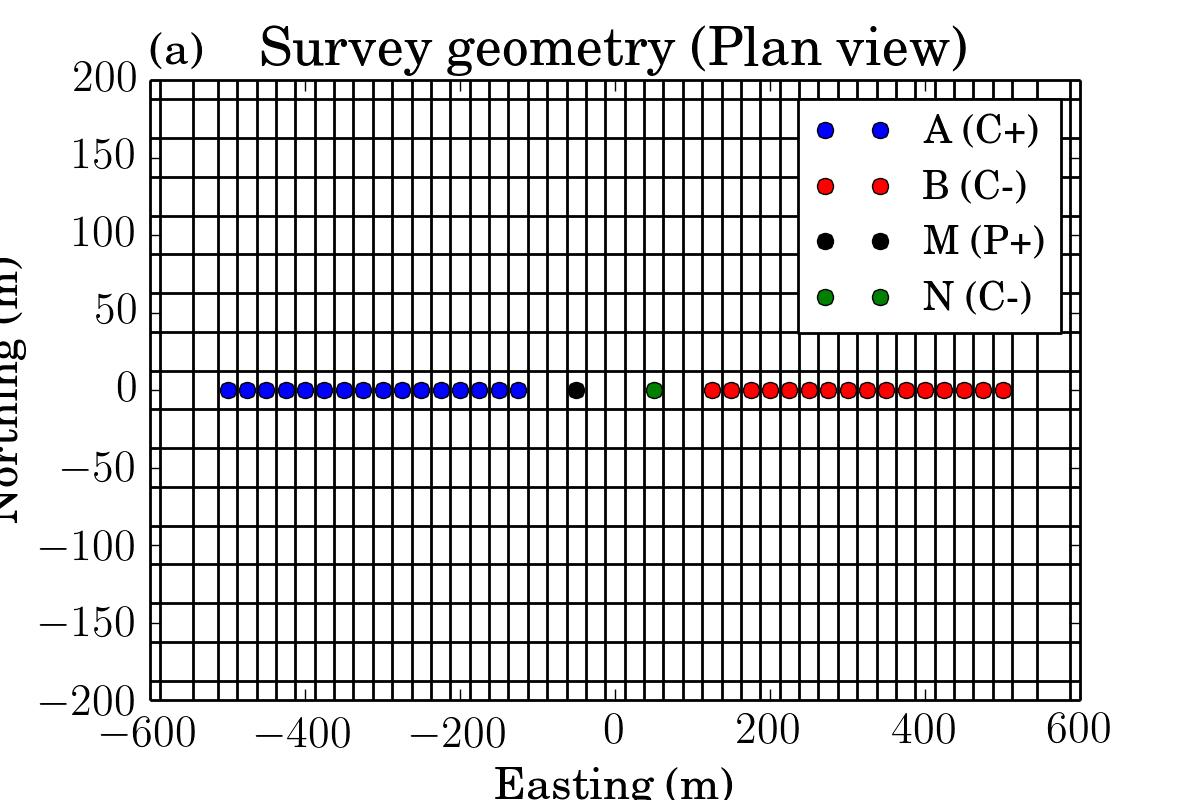
\includegraphics[width=7cm]{images/DCsurvey.png}
% 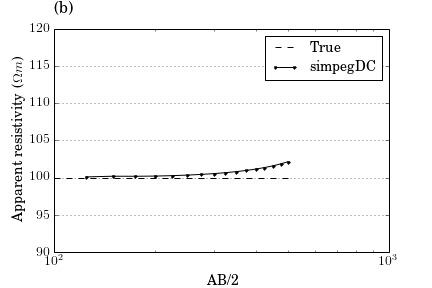
\includegraphics[width=7cm]{images/comp_dc.png}
% \caption{ (a) Survey geometry of Schlumbuerger array. (b) Comparison of true and computed apparent resitivity values.}
% \label{fig:DCfwd}
% \end{figure}

\subsection{Sensitivities}
The sensitivity and adjoint will be used in the optimization routine of the inversion.
Inefficient or inaccurate calculation of the sensitivities can lead to an extremely slow inversion.
This is critical in large-scale inversions where the dense sensitivity matrix may be too large to hold in memory directly.
As discussed in the methodology section, the sensitivity matrix need not be explicitly created when using an
iterative optimization algorithm such as Gauss-Newton (\ref{eq:gn}) solved with a conjugate gradient approach.
The calculation of vector products with the sensitivity matrices is an important aspect of \SimPEG,
which has many tools to make construction and testing of these matrices modular and simple.
For the DC resistivity example, the discretized governing equations are written as $C(\mathbf{m},\mathbf{u}) = \bf A(\m)\u - q = 0$.
We can implement the sensitivity equations \ref{eq:J} and \ref{eq:dcdm_dcdu_rearranged} to yield:
{%\iftoggle{finaldraft}{
\begin{equation}
\mathbf{J} = - \mathbf{P}(\mathbf{A}(\m)^{-1} \nabla_\m C(\m,\u)),
\end{equation}
}
where $\nabla_\m C(\m,\u)$ is a known sparse matrix,
$\bf A(m)$ is the forward operator and is equivalent to $\nabla_\u C(\m,\u)$,
and $\bf P$ is a projection matrix (cf. \cite{Pidlisecky2007}).
Each matrix in this expression is sparse and can be explicitly formed, however,
the product is dense and it may not be possible to hold it in memory. If an iterative
solver is used in the optimization, only matrix vector products are necessary and
the sensitivity need not be explicitly calculated or stored.
Figure~\ref{fig:dcSensitivity} outlines the calculation of \texttt{Jvec}
given a model, \texttt{m}, the fields, \texttt{u}, and a vector to multiply, \texttt{v}.
In Figure~\ref{fig:dcSensitivity}, we draw the distinction between the model, \texttt{m}, and
the conductivity, \texttt{sig}, which are connected through a mapping, $\sigma = \mathcal{M}(\m)$, and associated derivatives.
The matrix $\nabla_\m C(\m,\u)$ is denoted \texttt{dCdm} and formed by looping over each
source in the DC resistivity survey.

{%\iftoggle{finaldraft}{
\begin{figure}[ht!]
\centering
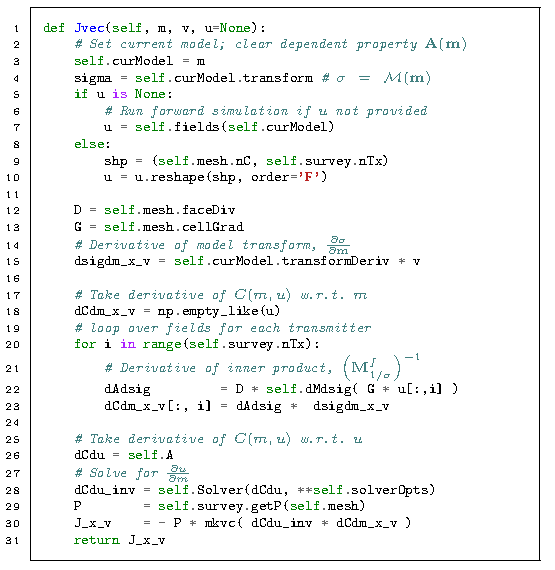
\includegraphics[width=7.5cm]{DC_Jvec_function.pdf}
\caption{Sensitivity times a vector method for the \DCProblem.}
\label{fig:dcSensitivity}
\end{figure}
}

%%%%%%%%%%%%%%%%%%%%%%%%%%%%%%%%%%%%%%%
%%%%%% Start Inversion Section!! %%%%%%
%%%%%%%%%%%%%%%%%%%%%%%%%%%%%%%%%%%%%%%

\subsection{Inversion elements}

As indicated in the methodology section, there are two key elements needed for
a geophysical inversion: \DataMisfit and \Regularization.
The \DataMisfit must have a way to calculate predicted data, as such, it takes a paired
survey as an initial argument, allowing forward simulations to be completed.
\DataMisfit and \Regularization have similar interfaces which are shown in Table~\ref{table:Dmis_and_Reg}.
The \DataMisfit class also has a property, \texttt{targetMisfit}, for the target misfit, which
can be checked by an \texttt{InversionDirective} and used as a stopping criteria.
As discussed in the methodology section, the \Regularization is defined independently
from the forward simulation. The regularization is with respect to the model, which may or may not be on the same mesh as the forward simulation (i.e. \meshI $\ne$ \meshF).
In this case, a mapping of a model to a physical property on the forward simulation mesh is necessary for the \Problem.
The \Regularization class also has a \texttt{mapping} property allowing a wide variety of regularizations to be implemented (e.g. an active cell map used to ignore air cells).
As such, the \Regularization \texttt{mapping} is often independent from the \texttt{mapping} in the \Problem class, which outputs a physical property.
Included in the \SimPEG package are basic Tikhonov regularization routines and simple
$l_2$ norms for both \Regularization and \DataMisfit classes.
Each of these classes has properties for the appropriate model and data weightings discussed in the previous section (e.g. $\Wm$ and $\Wd$).
These classes are readily extensible such that they can be customized to specific problems and applications, such as considering $l_1$ or $l_p$ norms or customized regularizations.

{%\iftoggle{finaldraft}{
\begin{table}[ht]
\caption{Common functions for the \Regularization, \DataMisfit, \InvProblem classes.}
\scriptsize
\label{table:Dmis_and_Reg}
  \begin{tabular}{  p{2.5cm}  p{4.5cm} }
    \hline

    Function & Explanation \\ \hline

    eval(m)          & Evaluate the functional given a model.\\
    evalDeriv(m)     & First derivative returns a vector.\\
    eval2Deriv(m, v) & Second derivative as an implicit operator.\\

    \hline
  \end{tabular}
\end{table}
}

\subsection*{Inverse Problem and Optimization}

The \InvProblem combines the \DataMisfit and \Regularization classes by introducing a
trade-off parameter, $\beta$. In addition to the trade-off parameter, there are
methods that evaluate the objective function and its derivatives (Table~\ref{table:Dmis_and_Reg}). Additional methods can save fields
such that information is not lost between evaluation of the objective function and the derivatives.
The \InvProblem may also include bounds on the model properties so they can be used in the optimization routine.
If one considers a joint or integrated inversion, multiple data misfit functions, employing different physics, and multiple types of regularization functionals may be summed together, possibly with relative weightings, to define the \InvProblem (cf. \cite{lines1988cooperative,Holtham2010,HeagySEG2014}).
Once the \InvProblem can be evaluated to a scalar and has associated derivatives, an \Optimization can either be chosen among the ones included in \SimPEG or provided by an external package.
Optimization routines in \SimPEG include steepest descent, L-BFGS, and Inexact Gauss-Newton (cf. \cite{Nocedal1999}).
The components are relatively simple to hook up to external optimization packages, for example, with the optimization package in SciPy \citep{scipy}.

\subsection{Inversion}

The \Inversion conducts all communication between the various components of the framework
and is instantiated with an \InvProblem object.
The \Inversion has very few external methods, but contains the list of directives that are executed throughout the inversion.
Each \texttt{InversionDirective} has access to the components of the inversion framework and can thus access and change any of these components as the inversion is running.
A simple directive may print optimization progress or save models to a database.
More complicated directives may change or compute parameters such as $\beta$, reference models, data weights, or model weights. These directives are often guided by heuristics, but versions can often be formalized, see for example the iterative Tikhonov style inversion \citep{tikhonov1977solutions,parker1994geophysical,DougTutorial}.
There are many computational shortcuts that may be investigated, such as how many inner and outer CG iterations to complete in the inexact Gauss-Newton optimization and whether this should change as the algorithm converges to the optimal model.
The \texttt{directiveList} in the \Inversion encourages heuristics that geophysicists often complete `by hand' to be codified, combined, and shared via a plug-in style framework.

\subsection{DC resistivity inversion}

We will build on the example presented in Section~\ref{sec:DCforward}, which has a survey setup that only provides enough information for a vertical sounding.
As such, we will decouple our 3D forward mesh and 1D inversion mesh and connect them through a mapping (cf. \cite{KangSEG2015}).
Additionally, since electrical conductivity is a log-varying parameter, we will also construct a model space that is optimized in log space.
Both of these model transformations will be handled with a single map, $\mathcal{M}$, where $\boldsymbol{\sigma} = \mathcal{M}(\mathbf{m})$.
{%\iftoggle{finaldraft}{
{\scriptsize\begin{verbatim}
    from SimPEG import Maps
    mapping = Maps.ExpMap(mesh) * Maps.Vertical1DMap(mesh)
    sigma = mapping * model
\end{verbatim}}
}
\noindent
We have provided a number of common mapping transformations in the \texttt{SimPEG.Maps} package, and these can be easily combined through a
multiplication symbol. Additionally, when using these maps, the derivatives are calculated using the chain rule allowing them to be easily
included in the sensitivity calculation (cf. Figure \ref{fig:dcSensitivity}, line 15). Figure~\ref{fig:DCinverse} demonstrates this mapping visually.
The 1D model is in $log(\boldsymbol{\sigma})$, shown in Figure~\ref{fig:DCmapping}(a) as a black solid line and the transformation produces a 3D \texttt{sigma} vector which was plotted in Figure~\ref{fig:DCmapping}(b). We can now use the same simulation machinery as discussed in Section~\ref{sec:DCforward}, with a single change:
{%\iftoggle{finaldraft}{
{\scriptsize\begin{verbatim}
    problem = DC.ProblemDC(mesh, mapping=mapping)
\end{verbatim}}
}

Synthetic data, $\dobs$, are created using the 1D log-conductivity model and adding 1\% Gaussian noise.
When creating the regularization inversion element, again we note that the \texttt{mapping} parameter can be used to regularize in the space which makes the most sense. In this case we will regularize on a 1D mesh in log-conductivity space, as such, we supply only a 1D tensor \texttt{mesh} to the regularization.
An inversion is run by combining the tools described above. Figure~\ref{fig:classOutline} illustrates how the components are put together.
{%\iftoggle{finaldraft}{
{\scriptsize\begin{verbatim}
    mesh1D  = Mesh.TensorMesh([mesh.hz])
    dmis    = DataMisfit.l2_DataMisfit(survey)
    reg     = Regularization.Tikhonov(mesh1D)
    opt     = Optimization.InexactGaussNewton()
    invProb = InvProblem.BaseInvProblem(dmis, reg, opt)
    inv     = Inversion.BaseInversion(invProb)
    mopt    = inv.run(m0)
\end{verbatim}}
}
\noindent
We note that there are many options and inputs that can enhance the inversion; refer to the online up-to-date documentation (http://docs.simpeg.xyz). The result of this inversion can be seen in Figure~\ref{fig:DCinverse}(a) and (b) for the predicted data and model, respectively.

{%\iftoggle{finaldraft}{
%DWO Captions  need to be expanded. Perhaps put all figures extending from (0,500)
\begin{figure}[ht!]
\centering
% 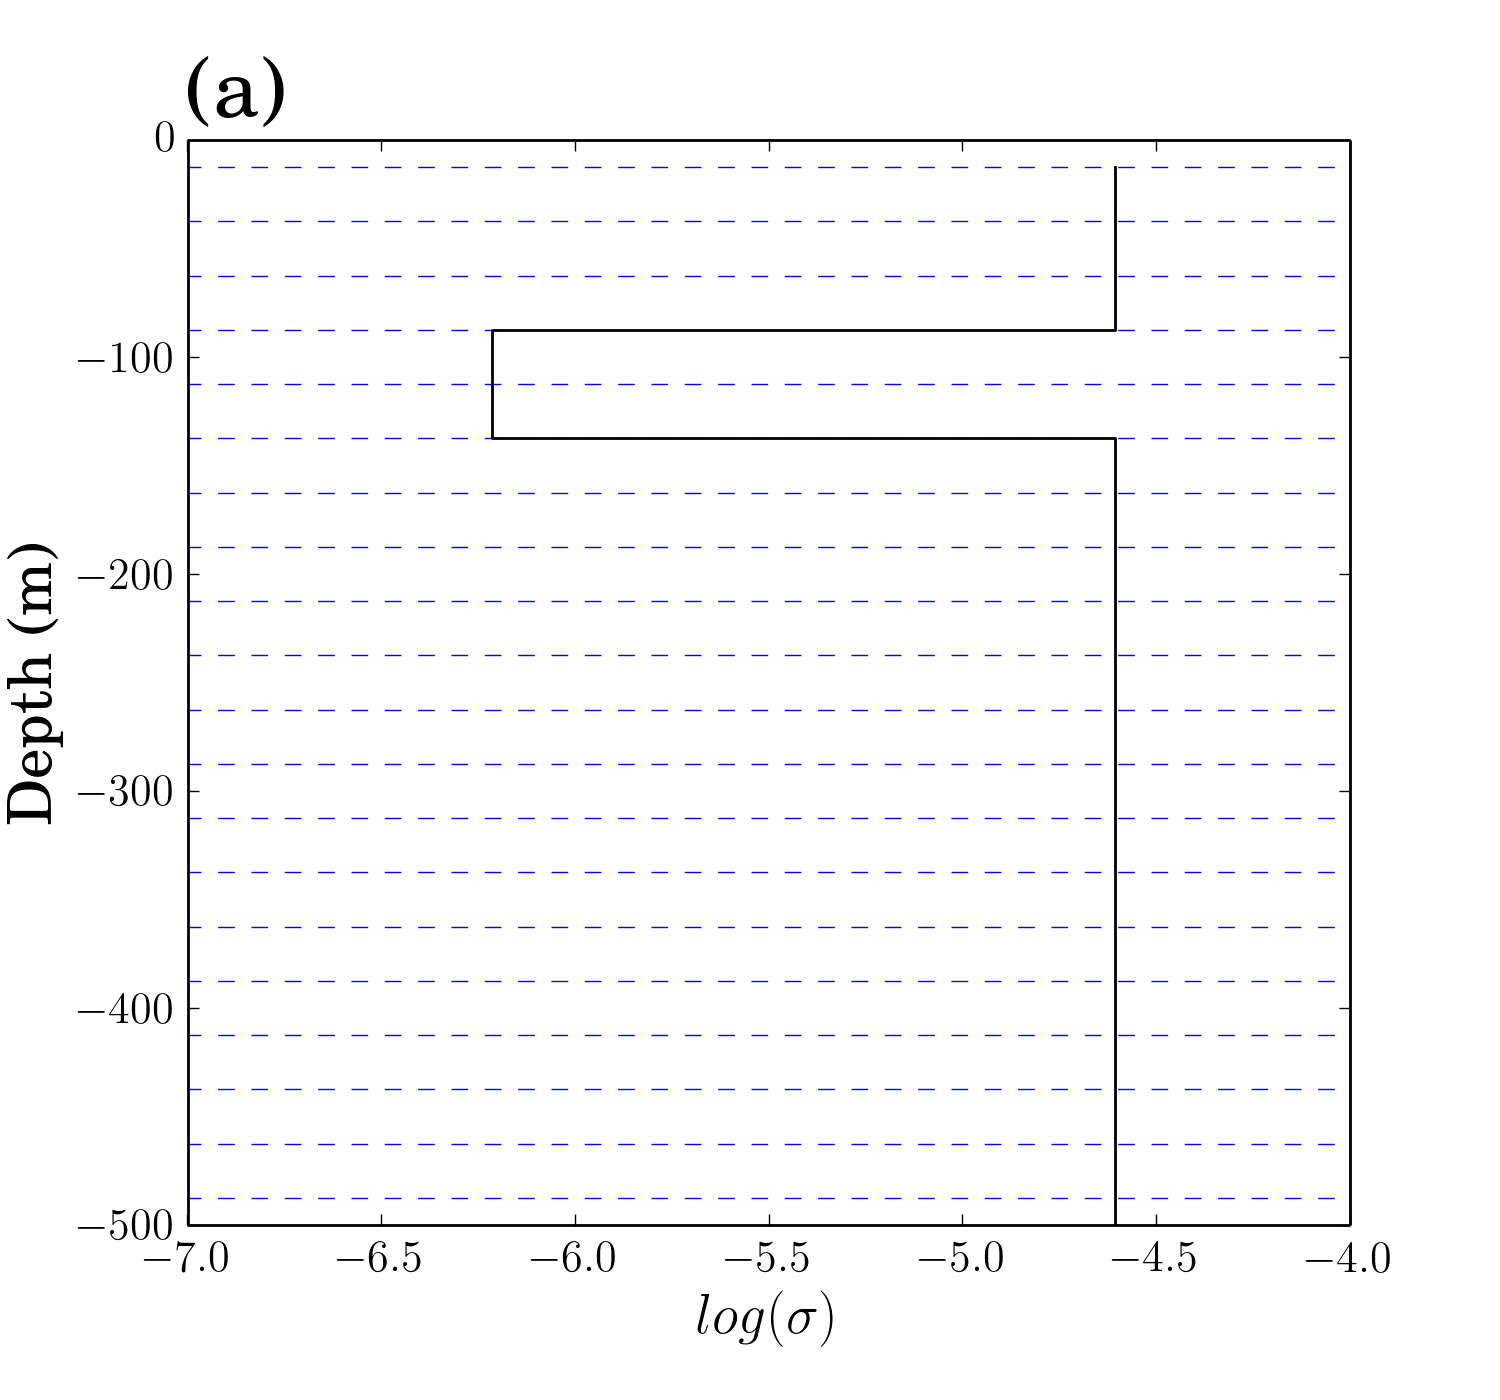
\includegraphics[width=5.4cm]{images/logcond1d.png}
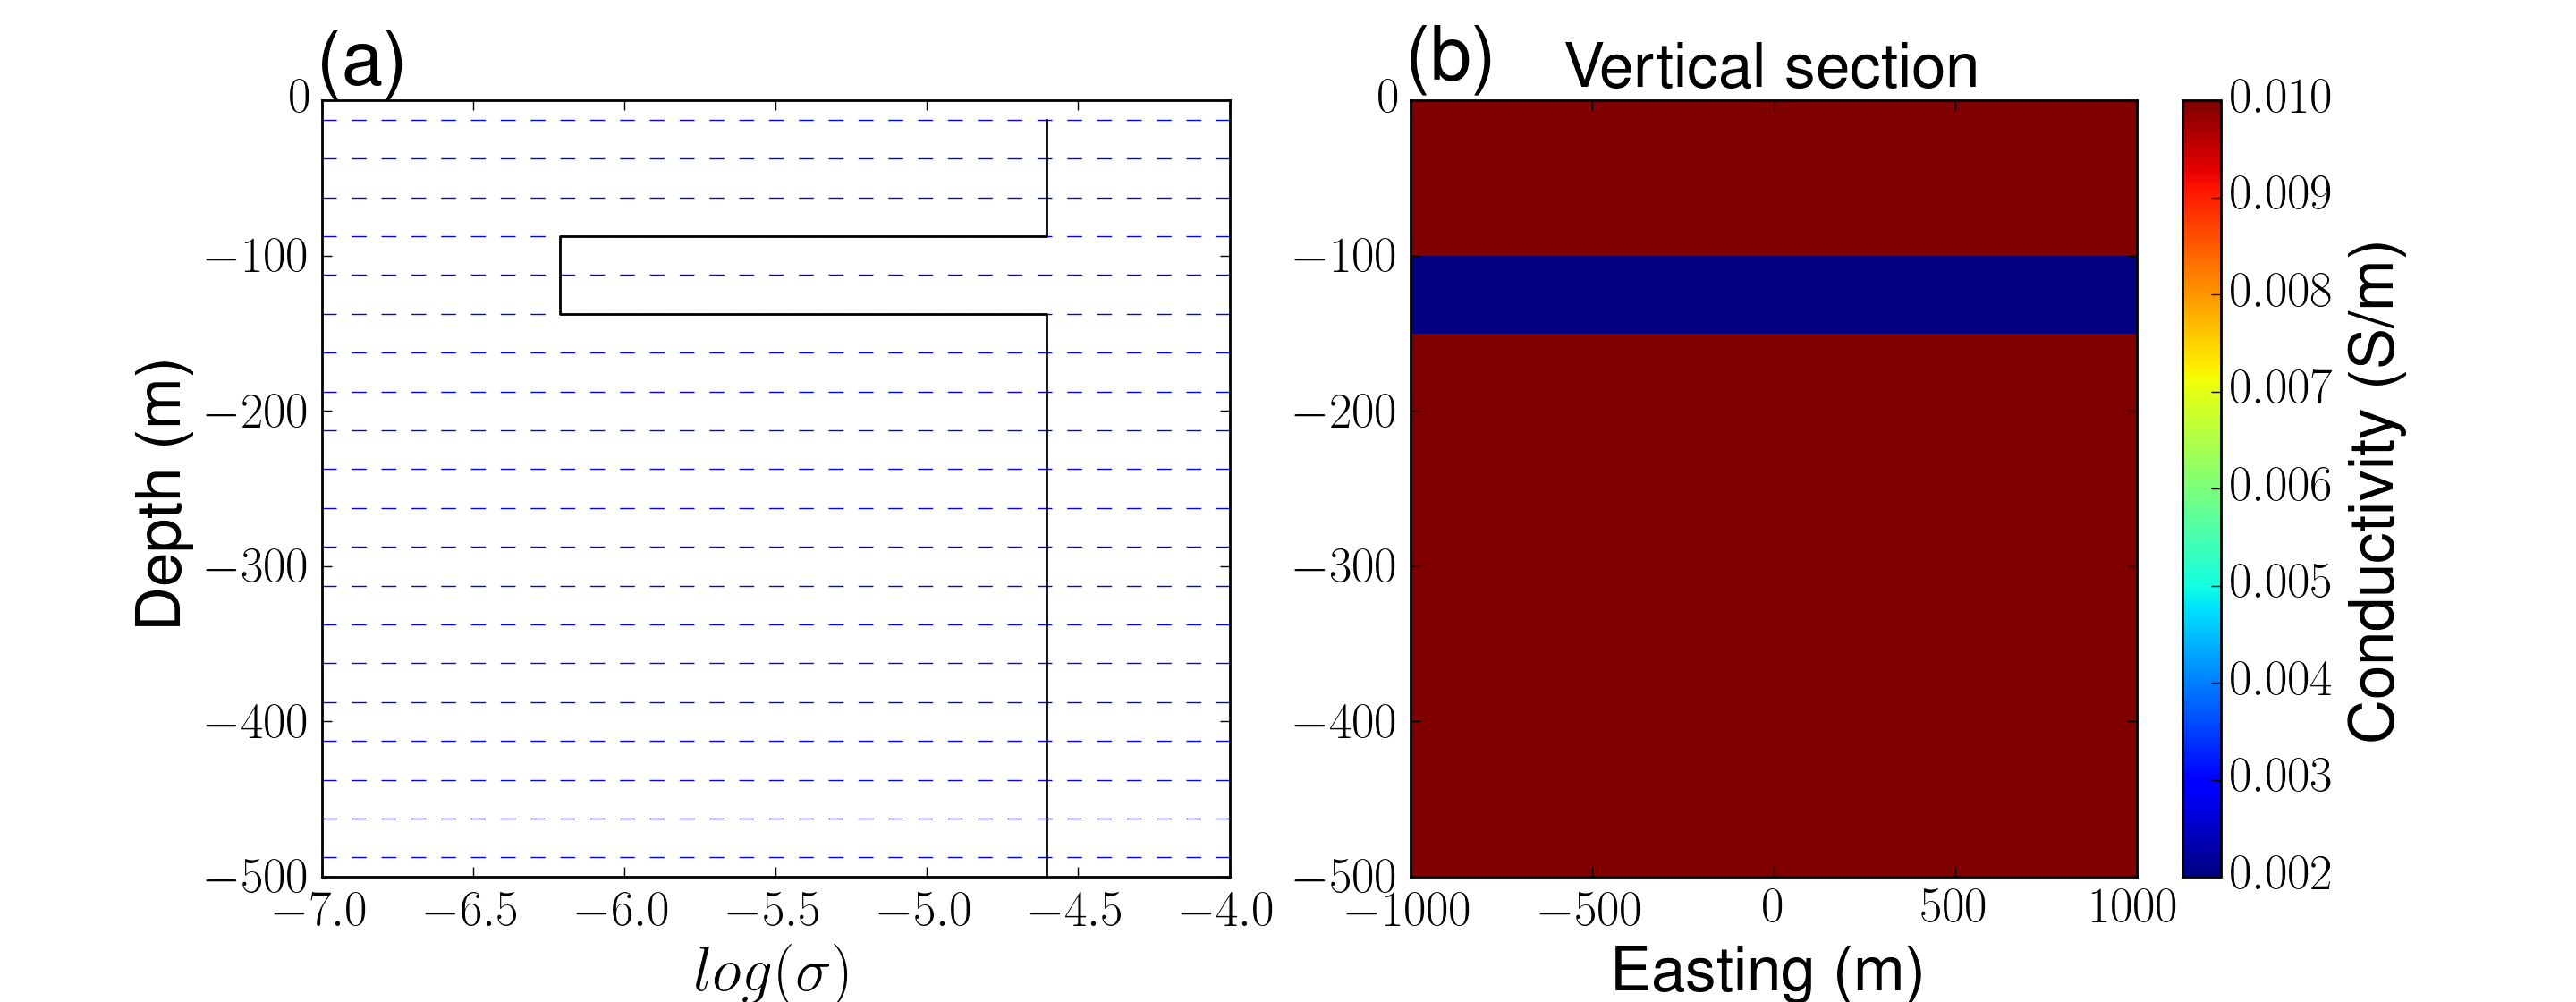
\includegraphics[width=16cm]{images/mappingDC.png}
\caption{Illustration of mapping in DC inversion. (a) 1D log conductivity model. (b) 3D conductivity model.}
\label{fig:DCmapping}
\end{figure}
\begin{figure}[ht!]
\centering
% 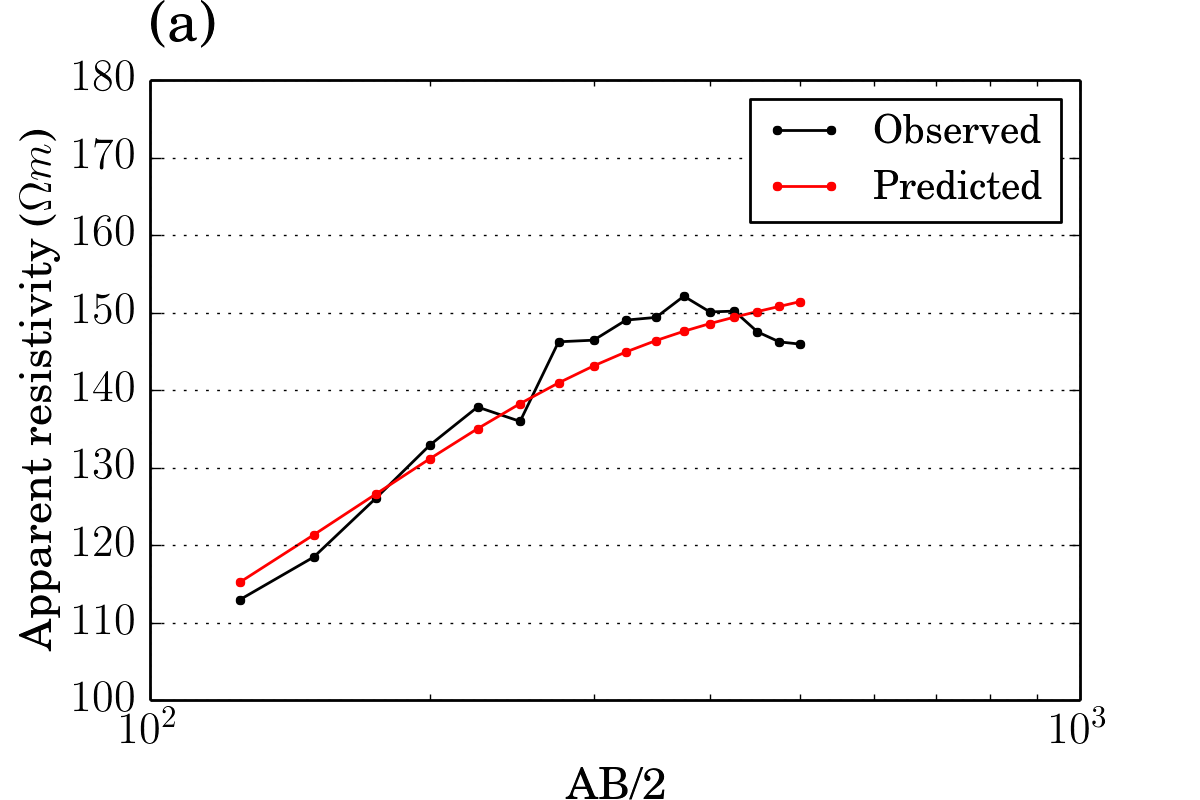
\includegraphics[width=7.5cm]{images/obspred_dc1d_dat.png}
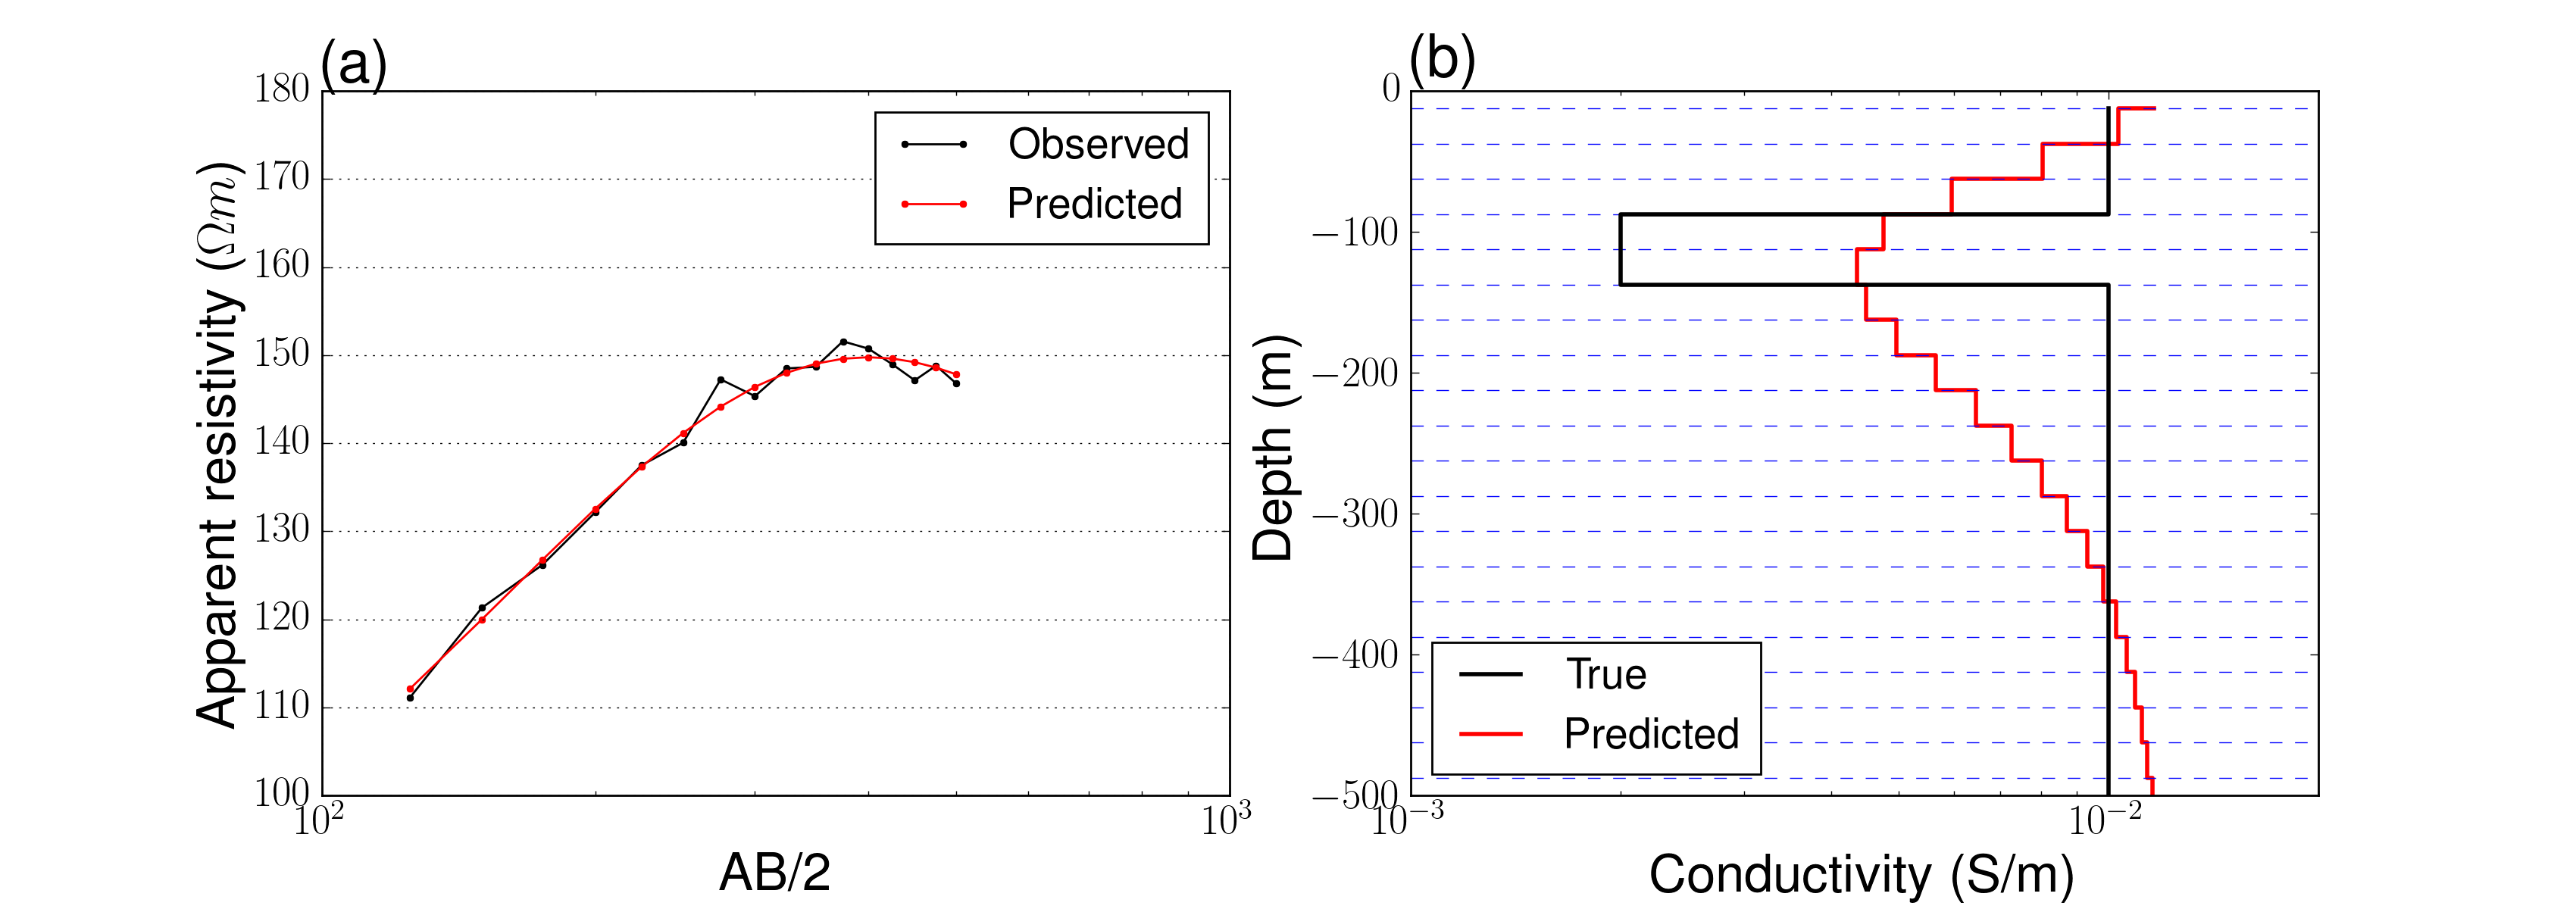
\includegraphics[width=16cm]{images/obspredDC.png}
\caption{(a) Observed (black line) and predicted (red line) apparent resistivity values. (b) True and recovered 1D conductivity model. }
\label{fig:DCinverse}
\end{figure}
}


\subsection{Development Practices}

Throughout the development of \SimPEG, we have focused on building both a framework (Figure~\ref{fig:classOutline}) and a toolbox that is flexible and extensible.
The toolbox includes utilities that we use repeatedly in our research, for example, visualization routines, mesh generation, and synthetic modeling.
Additionally, when writing new code for differential operators and PDE systems, several functions are available to help test and verify results including: (a) checking derivatives and expected order of convergence, (b) comparing to analytics, and (c) adjoint tests for the sensitivity operators (cf. \cite{haber2015computational}).
These tests can be written in-line in an interactive development paradigm and then rapidly transfered and incorporated as unit-tests to ensure future code changes do not change functionality.
Currently the entire \SimPEG project has upwards of 80\% test coverage,  with all core functionality (e.g. discretization, optimization) being extensively tested.
All changes are combined using the practice of continuous integration, supported by freely available tools for open source projects such as TravisCI and GitHub.
Additionally, we have focused on writing and maintaining documentation for core functionality (http://docs.simpeg.xyz). The documentation is also practicing continuous integration and is updated with all changes to \SimPEG and is built and hosted through ReadTheDocs \citep{RTFD}.
We are hopeful that our efforts and adherence to best practices in open source code development (cf. \cite{Wilson2014}) will encourage a community to exercise reproducible research around these scientific tools (cf. \cite{Fomel2009}).


\section{Conclusions}
\label{sec:conclusions}

Producing an interpretation from geophysical data through an inversion is an iterative process with many moving pieces. A number of inversion components, techniques and methodologies have become standard practice. The development of new methodologies to address the evolving challenges in the geosciences will build upon and extend these standard practices, requiring experimentation with and recombination of existing techniques.
To facilitate this combinatorial experimentation, we have organized the components of geophysical inverse problems in a comprehensive, modular framework. Our implementation of this framework, \SimPEG (http://www.simpeg.xyz), provides an extensible, well-tested toolbox and infrastructure that supports problems including electromagnetics, fluid flow, seismic, and potential fields. As \SimPEG is formulated with the inverse problem as its core focus, many design choices have been made to ensure that sensitivities are efficient to compute and are readily available; we presume this will be advantageous for integrated geophysical inversions. The modular framework we suggest splits the code into components that are motivated directly by geophysical methodology and terminology. This allows each piece to be improved by specialists whilst promoting quantitative communication between researchers.

To accelerate the dissemination and adoption of \SimPEG in the wider community, we have made the entire project open source under the permissive MIT License. The usability of this framework has been a focus of \SimPEG, and we strive to use best practices of continuous integration, documentation (http://docs.simpeg.xyz), unit-testing, and version-control. These practices are key to have in place as more modules and packages are created by the community.

{%\iftoggle{finaldraft}{
\section*{Acknowledgments}
% \label{sec:acknowledgments}
We would like to thank Dr. Eldad Haber for his invaluable guidance and advice in the development process of our framework and \SimPEG implementation.
Dr. Dave Marchant, Dr. Lars Ruthotto, Luz Angelica Caudillo-Mata, Gudni Rosenkjaer, and Dr. Brendan Smithyman
have contributed to the \SimPEG code base and are always willing to talk through problems and ideas.
The funding for this work is provided through the Vanier Canada Graduate Scholarships Program, and grants through
The University of British Columbia (NSERC 22R47082) and
the University of Calgary (NSERC Discovery Grant for A. Pidlisecky).
We also acknowledge and thank three reviewers, Peter Leli\`{e}vre, Thomas Hansen, and an anonymous reviewer for their thoughtful and constructive comments on this manuscript.

\newpage

% \section*{References}
\bibliographystyle{elsarticle-harv}
\bibliography{refs}
}

\end{document}
